\documentclass[11pt]{article}

\usepackage[utf8]{inputenc}
\usepackage{mathptmx}
\usepackage{amsmath}
\usepackage{amssymb}
% \usepackage{unicode-math}
% \setmathfont{latinmodern-math.otf}
\usepackage{multirow}
\usepackage{hyperref}
\usepackage[authoryear]{natbib}
\usepackage{enumerate}
\usepackage{longtable}
\usepackage{subcaption}
\usepackage{geometry}
\usepackage{booktabs}
\usepackage{tabularx}
\usepackage{lscape}
\usepackage{color}
\usepackage{dcolumn}
\usepackage{booktabs}
\usepackage{rotating}
\usepackage{supertabular}
\usepackage{tabulary}
\usepackage{graphicx}
\usepackage{ltablex}
\usepackage{setspace}
\usepackage{float}
\usepackage[stable]{footmisc}
\usepackage{graphicx}
\usepackage{todonotes}
\usepackage{nameref}
\usepackage[blocks]{authblk}% The option is for block layout
\usepackage{atbegshi}% http://ctan.org/pkg/atbegshi
\AtBeginDocument{\AtBeginShipoutNext{\AtBeginShipoutDiscard}}

% \usepackage[capposition=top]{floatrow} % Notes for figures
% \usepackage[textsize=tiny]{todonotes}

\newcommand{\ra}[1]{\renewcommand{\stretch}{#1}}

% caption format
\usepackage{caption}
\usepackage{varwidth}
\DeclareCaptionFormat{myformat}{%
  % #1: label (e.g. "Table 1")
  % #2: separator (e.g. ": ")
  % #3: caption text
  \begin{varwidth}{\linewidth}%
    \centering
    #1#2#3%
  \end{varwidth}%
}

\captionsetup{format=myformat}% global activation

% more on captions
\setlength{\abovecaptionskip}{5pt}   % 0.5cm as an example
\setlength{\belowcaptionskip}{5pt}   % 0.5cm as an example
% \setlength\parskip{11pt}
%\renewcommand{\sfdefault}{lmss}
%\renewcommand{\ttdefault}{lmtt}

% citation style
\setcitestyle{aysep={}}

% % Alter some LaTeX defaults for better treatment of figures:
% \renewcommand{\topfraction}{0.9}  % max fraction of floats at top
% \renewcommand{\bottomfraction}{0.8}  % max fraction of floats at bottom

% \setcounter{topnumber}{2}
% \setcounter{bottomnumber}{2}
% \setcounter{totalnumber}{4}     % 2 may work better
% \setcounter{dbltopnumber}{2}    % for 2-column pages
% \renewcommand{\dbltopfraction}{0.9} % fit big float above 2-col. text
% \renewcommand{\textfraction}{0.07}  % allow minimal text w. figs

% \renewcommand{\floatpagefraction}{0.7}  % require fuller float pages
% \renewcommand{\dblfloatpagefraction}{0.7} % require fuller float pages
% % remember to use [htp] or [htpb] for placement


% tables
\setlength{\tabcolsep}{10pt}
\setlength{\defaultaddspace}{.60ex} % space between numbers
\captionsetup{belowskip=12pt,aboveskip=8pt}
\renewcommand{\arraystretch}{1.15}

% siunitx

\usepackage{siunitx} % centering in tables
  \sisetup{
    detect-mode,
    tight-spacing   = true,
    group-digits    = false ,
    input-signs   = ,
    input-symbols   = ( ) [ ] - + *,
    input-open-uncertainty  = ,
    input-close-uncertainty = ,
    table-align-text-post = false
        }

% margins
\pdfpagewidth 8.5in
\pdfpageheight 11in

\setlength\topmargin{0in}
\setlength\headheight{0in}
\setlength\headsep{0in}
\setlength\textheight{9in}
\setlength\textwidth{6.5in}
\setlength\oddsidemargin{0in}
\setlength\evensidemargin{0in}
\setlength{\footskip}{.7in}
\setlength\parskip{11pt}


% citation style
\setcitestyle{aysep={}}

% % Alter some LaTeX defaults for better treatment of figures:
% \renewcommand{\topfraction}{0.9}  % max fraction of floats at top
% \renewcommand{\bottomfraction}{0.8}  % max fraction of floats at bottom

% \setcounter{topnumber}{2}
% \setcounter{bottomnumber}{2}
% \setcounter{totalnumber}{4}     % 2 may work better
% \setcounter{dbltopnumber}{2}    % for 2-column pag es
% \renewcommand{\dbltopfraction}{0.9} % fit big float above 2-col. text
% \renewcommand{\textfraction}{0.07}  % allow minimal text w. figs

% \renewcommand{\floatpagefraction}{0.7}  % require fuller float pages
% \renewcommand{\dblfloatpagefraction}{0.7} % require fuller float pages
% % remember to use [htp] or [htpb] for placement

\providecommand{\tightlist}{%
  \setlength{\itemsep}{0pt}\setlength{\parskip}{0pt}}



%%%%%%%%%%%%%%%%%%%%%%%%%%%%%%%%%%%%%%%%
% start document
%%%%%%%%%%%%%%%%%%%%%%%%%%%%%%%%%%%%%%%%

\begin{document}

%TC:ignore

\title{Income Mobility, Income Inequality and Mortality in the U.S.}

\author{Sebastian Daza}
\affil{Center for Demography and Ecology \\University of Wisconsin-Madison \\
\url{sdaza@ssc.wisc.edu}}

\author{Alberto Palloni}
\affil{Center for Demography and Health of Aging  \\University of Wisconsin-Madison \\
\url{palloni@ssc.wisc.edu}}

% \author{Elizabeth Arias}
% \affil{Mortality Statistics Branch, Division of Vital Statistics \\ National Center for Health Statistics \\
% \url{efa3@cdc.gov}}

% \author{Ezekiel J. Emanuel}
% \affil{Perelman School of Medicine and The Wharton School \\University of Pennsylvania}
% \url{sdaza@ssc.wisc.edu}}

\date{\parbox{\linewidth}{\centering%
  \today\endgraf\bigskip\bigskip\bigskip\bigskip\bigskip
  % Words: 7200
  }}

\thanks{Preliminary draft. The research on which this paper is based was supported by the National Institute on Aging via research project grants (R01 AG016209 {[}PREHCO{]}, R03 AG015673, R01 AG018016,
and MERIT award R37 AG025216), and by a Fogarty International Center
award for Global Research Training in Population Health (D43 TW001586).
The University of Wisconsin-Madison researchers are supported by core
grants to the Center for Demography and Ecology, University of Wisconsin
(R24 HD047873) and to the Center for Demography of Health and Aging,
University of Wisconsin (P30 AG017266).}

\begin{titlepage}
       \maketitle
\thispagestyle{empty}
\end{titlepage}


\thispagestyle{empty}
% \doublespacing
\section*{Abstract}

We assess the magnitude of the association between intergenerational income mobility and US adult mortality by gender, age group, race/ethnicity and the causes of death. We use a data set from \textit{The Health Inequality Project} and \text{CDC mortality} data at the county level. We find that under different model specifications the association between income mobility and adult mortality is strong, properly signed, and consistent with our hypotheses. If the association we find reflects a causal effect it would translate into shifts in life expectancy at age 40 of as much as 2.0-4.8 years among males and 0.1-2.0 among females, equivalent to 5.1-12.5 and 0.2-4.7 percent of the U.S. male and female life expectancy at age 40 respectively. On average, these effects are 1.5 to 2.5 times as large as those of income inequality and represent between 40 (males) and 25 (females) percent of the magnitude of an income shift from the lowest to the highest quartile of the U.S. income distribution. to the highest quartile of the U.S. income distribution.

\newpage
\setcounter{page}{1}

%TC:endignore

\section{Introduction}

Over the last ten years or so, there has been a steady increase of empirical evidence documenting large gaps in life expectancy at birth by geography in the US (state, counties), \citep{Murray2006, Ezzati2008}. These contrasts are not accounted for by differences in access to medical care, places' infrastructure or community characteristics, ethnic composition or, surprisingly,  places' income \citep{NationalAcademyofSciences2015}. This is remarkable in view of the fact that recent research shows that there are massive contrasts in adult mortality by income across US counties. In fact, the best performing counties in the U.S. have levels of life expectancy that are \textit{20 years larger than the poorest performer}. Moreover, there are indications that these disparities are expanding over time as the difference in life expectancy (at age 40) between the richest and poorest quartiles of the income distribution of US counties grew from 9 years to about 11 among men and from 5.2 years to 6.6 years among women \citep{Chetty2016}. These gaps are non-trivial and represent 25\% of life expectancy at age 40 among men and 13\% among women. Based on this evidence it would have been reasonable to expect that most, if not all, US geographic disparities vanish after accounting for place's income. But that's not the case. Evidently, other things matter as much or more. 

Steady or growing disparities in longevity by geography and by markers such as education and income present a unique challenge. They are odds with expectations about the role and influence of modern medicine and health care as well as with universally accepted norms of fairness. This may explain the large amount of research dedicated to find root causes of these disparities and to translate such knowledge into interventions directed at reducing them. An important part of this effort has been allocated to understanding the role of a place's income inequality. There is a large body of  literature that documents the existence of a positive association between levels of aggregate income inequality and poor health and mortality, particularly among individuals in the upper and lower part of the income distributions for countries, small areas, and individuals \citep{Pickett2015, SubraKawa2004,Wagstaff2000, WilkPick2006, WilkPick2009a, Kawachi1997,Wilkinson1992, DalyWilson2013, Wilkinson2009}. Emphasis on the potential role of income inequality has been buttressed by recent evidence documenting a steady increase in the US income inequality \citep{Piketty2003}, a fact that makes plausible the idea that recent increases in mortality disparities by geography could indeed be partially rooted in income inequality.

In this paper, we suggest that an understudied factor, income mobility, could also play a significant role. We argue that communities with low income mobility may host conditions that diminish opportunities for individuals' advancement and lifetime achievement, discourage forward looking strategies and careful planning, and weaken individuals' motivation to adhere to behaviors that minimize accumulation of exposure to health risks and could contribute to excess mortality across a broad spectrum of ages and  causes of death. Although both income inequality and income mobility are aggregate dimensions of a stratification system, they are quite distinct and should have different implications and impacts. Individuals in communities characterized by comparable levels of income and income inequality but faced with opposite lifetime income mobility prospects may be exposed during formative years to different learning experiences, preferences, and behavioral strategies that ultimately shape health behaviors and lifelong exposure to health risks. 

While the association between income inequality and health has been studied as part of a 20-year old literature, recent work suggests that its contribution to the explanation of disparities in longevity may be quite small \citep{Palloni2016, Murray2006, Ezzati2008}. In contrast, the health consequences of income mobility have been rarely studied, a surprising fact in light of growing empirical evidence of a long-term decline in intergenerational social and income mobility in the US among the birth cohorts currently experiencing increased mortality disparities \citep{Chetty2017, Hout1993, Hout1988, Hout1984}. This research landscape is changing and in a series of very recent papers, a group of researchers began exploring the association between a place's income mobility and health behaviors, self-reported health and mortality. \citep{Venkataramani2015,Venkataramani2016,Palloni2016}. 

The goal of this paper is to extend this emerging area of study. First, we propose, but are not able to rigurously test for, pathways through which income mobility may influence individuals' health and mortality. These pathways are distinct from, albeit related to, those associated with income and income inequality, operate independently of these, greatly overlap with pathways that enhance adult labor market success, and could potentially have powerful impacts on health and mortality disparities across socioeconomic and race groups.Second, we test selected, well-defined but inevitably narrow hypotheses about expected patterns of association between income mobility and adult mortality. Third, we compare the magnitude of associations between income mobility and mortality and income inequality and mortality. Fourth, we estimate age, race/ethnic, and cause-of-death specific patterns of associations. Fifth, we compute potential losses/gains of years of adult life resulting from shifts in aggregate income mobility. 

Our results suggest that places with higher levels of income mobility also experience lower adult mortality risks and that these impacts are larger than those attributable to a place's income inequality. The age pattern of effects contains a peak in young to middle adulthood and becomes attenuated at very old ages.The association is similar for males and females but stronger among African American population. Finally, we find that the excess mortality associated with lower income mobility is mainly due to the influence of communicable diseases, accidents and injuries.

% We also find that the association is stronger among men than among females, more salient in the age groups 20-69. 
We argue that communities with high income mobility share characteristics that help individuals and families manage resources available to them, improve resilience to adverse conditions and, ultimately, reduce individual exposure to health risks, irrespective of a community's income level and income inequality. We hasten to add that, like other recent findings, ours are all about associations, do not prove causality and could be accounted for a number of alternative interpretations regarding the mechanisms that produce them.\footnote{Throughout the paper we use the term \textit{effects} to refer to the magnitude and sign of standardized or non-standardized regression coefficients measuring the strength of the relation between two variables and do not presume the existence of a proven causal relationship.}

% Economic mobility – defined as the ability of individuals to exceed the income of their parents – may play an important role in explaining these disparities. 

% We used newly available, local-area level data on income-specific life expectancy and social mobility to assess the relationship between income mobility and longevity by gender, age, race/ethnicity and cause of death.  We also assessed the extent to which differences in economic mobility may contribute to income gaps in longevity.

\section{The relation between aggregate income mobility and mortality}

We begin with a disclaimer about what our goal is not. Although relevant, we do not study the effect of \textit{individuals' income mobility} on their own health and mortality risks. There is a large and distinguished body of research in epidemiology on the relations between individuals' lifetime mobility and their adult mortality \citep{Chandola2003, Illsley1955, Fox1982, Blane1999, Blane1993}. The bulk of this literature is concerned with the long run impact of early occupational (career) shifts or the short run effects of late occupational (career) shifts. This work is based on empirical research that focuses on patterns of relationships between individuals occupation (or SES status broadly conceived) at an early point in their adult life and subsequent older adult health and mortality. 

In contrast, our goal is to clarify the relation between a place's income mobility regime and individual mortality. Much as is the case for the study of income inequality and health and mortality, our focus is on the association between an \textit{aggregate} property of the stratification system and individual experiences. It is, of course, possible that individuals' experiences of occupation or SES mobility are also influenced by the prevailing regime of income mobility. Indeed, these experiences may be one of many other pathways through which aggregate income mobility and individual mortality are related. In this paper we are interested in the \textit{total} effects of places' income mobility on individual health and mortality and are not concerned with the precise empirical identification of mediating pathways (see below).

An association between income mobility and mortality could exist if communities with higher income mobility host social and economic environments that reduce mortality risks relative to communities with lower income mobility, \textit{independently of effects of income levels and income inequality}. Individuals and groups who occupy the most vulnerable and exposed social positions within unequal communities may be comparatively better off when they face advantageous income mobility prospects than when they do not. Just as individuals who command lower incomes in communities with more equitable income distributions may experience better health than individuals with similar incomes in societies with higher income inequality, so too could individuals and groups that occupy lower ranked positions in societies with higher income mobility enjoy better health than counterparts in societies with more rigid stratification systems. In theory, communities could be classified in one of the four cells in Table \ref{theoretical_scenarios}. Each cell in the table is characterized by a health and mortality profile. In view of the moderate-to-strong relation between income inequality and income mobility \citep{Palloni2016} we take it for granted that the frequency of observations is non-zero in all cells and that communities simultaneously characterized by unequal income distribution and flexible mobility regimes or by generous income distributions and high levels of social rigidity, are observable. The standard conjecture is that indicators of mortality and health will be more beneficial in communities with less inequality (B and D) than in those with high inequality (A and C). The new conjecture is that at a given level of income inequality, better health and mortality conditions will be experienced by members of communities with higher income mobility, A versus C, on one hand, and B versus D, on the other.

\subsection{Mechanisms}

We identify four pathways linking income mobility and mortality that seem highly plausible even though the empirical evidence assembled here is too coarse and can neither confirm their operation nor help us establish their importance relative to other, equally plausible ones. 

\subsubsection{Individual mobility experiences and adult health and mortality}

As stated above an association between aggregate income mobility and individual health and mortality may be the outcome of a composition effect, namely, places with higher income mobility contain a population composition biased toward individuals who experience mobility (and their health and mortality consequences). In this case, the association between the aggregate property of the stratification system and individual experiences of health and mortality reflects the influence of individual mobility patterns (and associated selection processes).

\subsubsection{Individual early experiences}

A large body of literature on health and mortality disparities demonstrates that SES (income, education), health and mortality gradients are pervasive, persistent and, as of recent, increasing everywhere in high-income countries \citep{MacKenbach2012, Meara2008}. Further, there is evidence that early conditions and upbringing of individuals matter greatly for adult health and mortality disparities \citep{Palloni2009,Case2002}. Thus, some of the health differentials between men in low and high ranking positions initially attributable to chronic stress among those in subordinate positions \citep{Marmot2004a, Sapolsky2005} may be rooted in antecedent health conditions sculpted early in life \citep{Case2011}. If early conditions are influential for SES health and mortality disparities, they may also be influential as vehicles that establish relations between income inequality, income mobility, and adult health and mortality. 

During early stages of socialization individuals experience sensitive and critical windows for the acquisition of cognitive and non-cognitive abilities that are the foundation of skills acquired later in life \citep{Knudsen.Heckman.ea2006, Shonkoff.Boyce.ea2009, Heckman2007, Cunha.Heckman2009}. Some of these traits involve the development of outlooks and attitudes that influence investments in skill acquisition and health, including propensities to adhere health-related behaviors. Thus, behaviors critically associated with modern chronic illnesses, such as smoking uptake and desistance, alcohol consumption, substance abuse, choices of diet and physical activity, are in part determined by capabilities sculpted early in life. Early avoidance of unhealthy behaviors has large payoffs in adulthood because these behaviors are closely related and reinforce each other, the physiological and psychological damage they produce are accumulated over time, and they all are strongly non-reversible. Early adoption of healthy behaviors is facilitated by socialization that emphasizes robust future outlooks, self-confidence, and self-reliance, beliefs in the neutrality and fairness of social reward allocation systems, hopefulness and optimism, and incentives to succeed. These are all traits that reduce time discounting so that the addition of one year of healthy life in the future of an individual is endowed with significant rewards and returns \citep{Grossman2000,Grossman1972}. 

We know from empirical research that negative affect, chronic stress, subordination, bleak future outlooks associated with poverty lead to increases in time discounting \citep{Haushofer2014}. Higher time preferences favors resistance to the adoption of behaviors that may yield immediate rewards but are health-damaging and discourage those that have a more distant and elusive pay-off but are health-preserving \citep{Schlam2013,Eigsti2006}.

We note that this mechanism alludes to influences that shape environments during critical stages of individuals' upbringing. The conjecture is that a places' income mobility regime is powerful enough to shape those environments. But so is an individual's ancestral income mobility experiences, particularly parental and possibly grand parental mobility. Strictly speaking these are two very different mechanisms that can be properly identified only if we simultaneously observe both the influences of a place's aggregate income mobility and individuals familial income mobility experiences.

\subsubsection{Community endowments}

Communities with low-income mobility may distort opportunities and incentives, reinforce unequal allocation of favorable traits, undervalue public institutions that contribute to the formation of skills with a high wage premium and, many of them, support non-meritocratic reward allocation strategies. These community properties directly influence the suite of opportunities available to individuals and shapes the way parents socialize children and favor (discourage) the adoption of positive outlooks and the value of skill acquisition. Rigid or weak income mobility fosters individual hopelessness, despair, mistrust, disbelief in a level playing field for all, weaken aspirations and, more generally, diminish the value of adoption of attitudes and behaviors that promote good health.

\subsection{Hypotheses}

The arguments above lead to some testable hypotheses:

\begin{enumerate}
    \item If any of the mechanisms identified above operate at all, one would expect that the association between a place's income mobility to which individuals are exposed early in life and their health and mortality as adults should be stronger in stages of the life cycle that reflect the impact of health relevant traits, for instance, during early adulthood and at older adult ages. In particular, we expect that exposure during formative years (between ages 5 and 20) to a particular income mobility regime will have stronger effects on mortality in age groups 15-49 and then after age 60.
    \item Causes of deaths contributing to excess mortality among individuals in low income mobility places should be associated with traits, preferences and behaviors that are sculpted early in life. Thus, for example, income mobility should have a larger impact on mortality due to chronic illnesses associated with smoking and diet among older adults and those associated with alcohol and drug use among younger adults, including outcomes such as suicides, homicides and other forms of violence.
    \item Deleterious effects of a rigid income mobility regime should be stronger among individuals who occupy low to low-middle income ranks than among those located in more favorable positions in the income ranking. Similarly, the effects should be larger among African Americans and other minorities that have been traditionally discriminated against and have access to a much-reduced set of opportunities relative to other groups in the population.
    \item  Gender differences should be muted if men and women are subject to similar expectations regarding social and economic accession. In contrast, in communities where families expect less from their daughters than from their sons and, more generally, whenever investments in sons exceed those in daughters, there should be stronger effects of a place income mobility among males than among females. \footnote{In the absence of suitable measures of gender preference or standards regarding gender's investment differentials, this hypothesis can only be crudely assessed.}
    \item Income mobility effects must be stronger in places with higher income inequality, that is in places where the health costs of income rigidity, particularly among those in the lower income ranks, are higher.
    \item Just as different regimes of income inequality may have their own repertoire of effects on health and mortality, different income mobility regimes have diverse health and mortality implications. For instance, inequality due to growth of the share of income in the top one percent of the income distribution has consequences that are quite different from inequality produced by increases in the share of the population in the lower income rank \citep{Piketty2003}. By the same token, income mobility regimes where the bulk of mobility is restricted to positions in the middle to upper part of the income distribution will have different repercussions than those in regimes where income mobility is concentrated among those in the low and middle-income ranks. 
    
    %  Even though ... explain our exercise assessing quintile transition matrices.
    
\end{enumerate}

In what follows, we examine the first five hypotheses. Empirical test of the last one requires richer information on mobility matrices than is currently available to us and is left for further research. 

\section{Data}

We use a large data set that results from merging of two separate data bases. The first is the Health Inequality Project Data (HIPD) created by Chetty and colleagues \citep{Chetty2016} that contains information on income from tax records for the period 1999 and 2014 by US counties and commuting zones. A total of 1.4 billion tax records were used and linked to Social Security Administration records. The HIPD include statistics of the income distributions and two indicators of income mobility derived from measures of the association between incomes of children born between 1971 and 1993 and their parents' income. We use the index of relative mobility (IRM), rank-rank slope, or the correlation between a child's income rank in her birth cohort income distribution and parents' income rank in their parents' income distribution.\footnote{Rank-rank slopes have proved to be quite robust across specifications and highly suitable for comparisons across areas \citep{Chetty2014}. \textit{Canonical} measures of relative mobility, such as inter-generational income elasticity (of child income with respect to parents' income) tend to be more sensitive to changes in inequality across generations.} The relative income mobility measure ranges between -1 and 1, and larger values correspond to lower income mobility (higher rank-rank correlation between parents' and child's income).  

We estimate our models using absolute upward mobility score or ``the mean rank (in the national income distribution) of children whose parents are at the 25\textsuperscript{th} percentile of the national parent income distribution'' \citep[p. 7]{Chetty2014}.\footnote{Although at the national level both the relative and absolute measure of mobility provide similar information, when studying small areas a child's rank in the national income distribution would be an absolute outcome because income in a given areas have little impact on the national distribution. We use a \textit{permanent-resident} version of income mobility measures, that is, parents who stay in the same counties between 1996-2012. Note that children who grow up in a county may have moved out as adults.}  Absolute upward income mobility ranges from 0 to 1, and higher values correspond to large income mobility. To facilitate interpretation we multiply the upward mobility score by -1 so that the meaning and expected association of relative and absolute income mobility with mortality are the same (i.e., increases in  income mobility and inequality is expected to rise mortality risk and viceversa). The results using absolute mobility are shown in the \nameref{sec:appendix} and they are similar to the ones using relative income mobility.\footnote{This is not surprising as the correlation between relative and absolute mobility scores is rather high (-0.70).} Finally, we use the Gini Index (GI) as an indicator of income inequality.\footnote{Gini coefficient within bottom 99\%.}
 
% In a separate paper \citep{Palloni2016}, we carried out extensive exploratory work of the relation between income mobility, income inequality, and mortality.

The second data base is the CDC mortality statistics by age and causes of death for U.S. counties during the period 2000-2014\footnote{Although the HIPD include coarse county mortality information, we use the CDC data for it enable us to compute rates by ages, sex, race/ethnic group, causes of death, and for periods of time that are better suited to the mobility data}. This includes detailed mortality statistics (death and population counts by age and cause of death) for periods of time that better match the period of reference of the income mobility indicator in the HIPD. We compute mortality rates by five year age groups starting at age 0. This ensures close correspondence to the observed income mobility experiences and minimizes the influence of systematic biases (see below). In addition, we are able to compute mortality by causes of deaths and thus test conjectures about patterns of effects of income mobility.

After merging the two data bases, we are able to include a total of 2867 counties, about 91\% of all counties in 2000 (see Figure \ref{fig:county_coverage} in \textit{\nameref{sec:appendix}}). We build different data modules tailored to the particular hypothesis we examine. Our more general model and analysis requires death counts aggregated by county and age group (51,606 records). We then add more complexity by \textit{disaggregating} the data by race/ethnic group and cause of death (about 200,000 records). 

Despite its richness, our data set has shortcomings. The most important one is the potential dislocation between exposure to an income mobility regime during formative years and mortality experiences. The CDC mortality information does not necessarily measure lifespans of people from places, but life spans of people who die in those places. Therefore, the associations we observe might be the result of selective migration over the life-course and not of exposures to a given mobility regime during critical ages. In other words, the effects of income mobility or inequality may be contaminated by characteristics that distinguish migrants from non-migrants. The only way to circumvent this is to use individual longitudinal data that provides enough information to either directly identify or to neutralize the effects of migration selection processes.

A second shortcoming is that even in the absence of residential migration, the measures of a place's income mobility does not correspond tightly to the mortality experience of interest. Thus, for example, a place's income mobility assessed for generations born in 1980 ought to be relevant for youth mortality in years (approximately) 1995-2010 and to older adult mortality for years 2040 and later. Lack of correspondence between income mobility and mortality is not problematic in a stationary regime, e.g., when a place's income mobility at time $t$ stays the same for a generation or so. The closer a place's income mobility is to a stationary regime, the stronger will be our inferences.

% The goal of this paper is to provide descriptives that help us to understand better the potential link between income mobility and mortality. This is just a first step into more... general... 

% First, the mortality experiences of each place correspond to older cohorts, parental and grad-parental, rather than to the children who were exposed during their formative years to each place's income mobility regimes. Second, the measure of mortality in the data, E(40), is obtained after extrapolation of a Gompertz function whose parameters are estimated using a fraction of the mortality experienced in adult years. Further, E(40) is a summary measure of mortality, mostly influenced by mortality rates over age 70, and can reflect radically different experiences of cohorts whose age is between 40 and 70 and those older than 70. Testing some of the hypotheses we propose requires more detail information on the age pattern of mortality.

% rather than 1559 in the HIPD data set.\footnote{This difference is accounted for counties with missing mortality data in the HIPD. The counties included in our analyses correspond to the continental US only as we exclude Alaska and Hawaii.}

\section{Model Estimation}

\subsection{General model and model estimation}

We seek to identify patterns of association between income mobility and mortality by county and demographic variables. First, we use death counts by county and age group as dependent variable. We fit Poisson models to the age group specific observed counts by gender with (midyear) population as offset. The most general model pools the death counts for all years (2000-2014), ethnicity/race, and causes of death available in the CDC data. Second, we include random effects for age groups as well as for state and county to capture unstructured associations of the death counts. Finally, we adjust for over-dispersion by adding a random effect at the observation level.\footnote{All random effects are assumed to be IID with mean 0 and variance $\sigma^2_{\varepsilon}$.}. The model is as follows:


\begin{align}
  D_{i} & \sim \text{Poisson}(\mu_i) \nonumber \\
 \text{log}(\mu_i) & = \text{log}(\tau_{i}) + \alpha + \beta_{ \text{m}} \text{M}_{i} + \beta_{\text{g}} \text{G}_{i} + \beta X_{i} \nonumber \\
    \alpha & =  \alpha_c + \alpha_{\text{state[i]}} + \alpha_{\text{county[i]}} +  \alpha_{\text{obs[i]}} + \alpha_{\text{age[i]}} \nonumber  \\ 
  \beta_{\text{m}}  & = \beta_{\text{Mob}} + 
  \beta_{\text{Mob}_{\text{age[i]}}} \nonumber  \\ 
   \beta_{\text{g}}  & = \beta_{\text{Gini}} + \beta_{\text{Gini}_{\text{age[i]}}} \label{eq:model_age}
\end{align}


% \begin{align}
%   D_{i} & \sim \text{Poisson}(\mu_i) \nonumber \\
%  \text{log}(\mu_i) & = \text{log}(\tau_{i}) + \alpha + \beta_{ \text{m}} \text{M}_{i} + \beta_{\text{g}} \text{G}_i + \beta X_{i} \nonumber \\
%     \alpha & =  \alpha_c + \alpha_{\text{state[i]}} + \alpha_{\text{county[i]}} \nonumber  \\ 
%   \beta_{\text{m}}  & = \beta_{\text{Mob}} + 
%   \beta_{\text{Mob}_{\text{state[i]}}} \nonumber  \\ 
%   \beta_{\text{g}}  & = \beta_{\text{Gini}} + \beta_{\text{Gini}_{\text{state[i]}}} \label{eq:model_general}
% \end{align}

\noindent where $D_i$ is the number of deaths by county and age, $\text{M}_i$ is the income mobility measure for county $i$, $\text{G}_i$ the Gini coefficient, and $\text{log}(\tau_i)$ is the logarithm of the exposure for county $i$ (i.e., log of mid-population). $X_i$ represents of a set of covariates we adjust for. Computing the exponential of $\alpha + \beta_{\text{m}} \text{M}_i + \beta_{\text{g}} \text{G}_i + \beta X_i$ yields the estimate of the mortality rate per county and age because $\text{log}(\lambda_i) = \text{log}(\mu_i) - \text{log}(\tau_i)$. $\alpha_{\text{obs[i]}}$ is the adjustment for overdispersion. In this model, the coefficients for income inequality (Gini index) and income mobility vary by age only. 

A few caveats are in order. First, in contrast to models with fixed effects using dummy variables for age groups (and corresponding interactions terms), the approach above allows for shifts in the estimates of age effects (and their corresponding confidence intervals) so that they are close to each other (partial pooling) where necessary. This is particularly important when, as happens in the CDC death statistics, information is sparse or when observed variation in the counts originates in noise. Fitting this type of multilevel model results in an important advantage, namely, it yields more reliable estimates for small groups and facilitate multiple comparisons \citep{Gelman2012, Hill2013}. 

Second, we extend the general model above by exploring interactions and expanding the data set by race/ethnic group and cause of death. Given the small number of categories being examined (four race/ethnicity and cause of death groups), we estimate  the model in Equation \ref{eq:model_age} separately for each race/ethnic/cause of death group. 

Finally, and most importantly, to circumvent shortcomings inherent to standard maximum likelihood estimates (MLE), we adopt a Bayesian approach and estimate the models with multiple nested and crossed random effects. All models are estimated with the integrated nested Laplace approximation (INLA, \citealt{Rue2009}), as this method does not require the use of simulation to sample from a posterior distribution thus facilitating the estimation relative to MCMC-based approaches.\footnote{For an applied introduction see \cite{Blangiardo2015, Wang2018} and \cite{Zuur2017}.}

To implement the Bayesian approach, we perform prior sensitivity analysis.\footnote{For more details see the \textit{\nameref{sec:sensitivity}} section in the \textit{\nameref{sec:appendix}}.} We start using the \texttt{R-INLA} default priors\footnote{\texttt{R-INLA} uses a precision measure for the variance of the posterior distribution parameters defined as $\tau_{\varepsilon} = \frac{1}{ \sigma^2_{\varepsilon} }$. The default prior distribution for a fixed parameter is a normal distribution with mean 0 and precision $\tau = 0.001$, that is equivalent to $\sigma = 31.62$. This diffuse prior is used for all fixed regression parameters, except for the intercept in which case the precision is 0, that is, the corresponding sigma is large. For parameterization of random effects \texttt{R-INLA} uses a log gamma distribution for the priors of $log(\tau)$ with shape $a = 1$ and inverse scale $b = 0.00005$.} and explore different specifications for Penalized Complexity (PC) priors which are designed to be weakly informative (for more details see \cite{Simpson2017}).  PC priors require we specify some scaling. To calibrate the scaling of the random effects prior, we set $U$ and $p$ to different values so that $Pr(\sigma_u > U) < p$. The values we use for $U$ and $p$, respectively, are PC(1,.10), PC(10, .10), PC(10, .0.1). In the first case, for instance, we calibrate the prior so that the probability that the standard deviation of the random effect is greater than 1 is lower than .10. Our main results are based on the PC prior that ensured better fit (e.g., \textit{deviance information criterion} (DIC) and \textit{Watanabe Akaike information criterion} (WAIC)), that is, PC(1, .10). Fortunately, estimates for income mobility and inequality are insensitive to different prior specifications. 

\subsection{Model variants}

We estimate six variants of the general model. The first is a baseline model that contains standardized income relative mobility (IRM), standardized income inequality (GI), centered log of the average household income and log of population at the county level as well as age, state, county, and observation level random-effects. Higher order models include income mobility and inequality age varying coefficients, interactions between income inequality and mobility, average income and corresponding interaction with IRM, and additional adjustments such as standardized income segregation, proportion of African-American (log), proportion of Hispanic (log), unemployment rate (log), proportion of people uninsured (standardized) and medicare expenses (standardized). All the variables were centered. \footnote{See Table \ref{tbl:descriptives} in the \nameref{sec:appendix} for descriptives of the variables we used.} Covariate adjustment could change estimates of the association between income mobility and mortality because they may capture unmeasured factors that confound the relationship of interest, but also because they reflect elements along a causal chain linking income mobility to health. Including covariates from the second group would amount to over-controlling and we intentionally sought to avoid this. For example, we do not include measures of health behaviors as covariates as it is likely that one of the pathways that relates income mobility and mortality includes changes in health behavior.\footnote{Goodness of fit of the covariate adjustment model using cross-validation is shown in the section \textit{\nameref{sec:gof}} in the \textit{\nameref{sec:appendix}}.}

Finally, we estimate models that consider spatial autocorrelation. Because county-level mortality data are area level information, spatial dependency is taken into account through neighborhoods structure. Neighbors are defined as the areas (counties) which share borders with it (first-order neighbors) or which share borders with it and with its first-order neighbors (second-order neighbors) \citep{Blangiardo2015}. We use the parameterization proposed by \cite{Riebler2016}. 

\subsection{Converting estimates of parameters into estimates of adult life expectancy}

To estimate effects of income mobility and income inequality on a summary measure of mortality, namely life expectancy at several ages, we use the parameter estimates of the model (Equation \ref{eq:model_age}) to compute predicted values of mortality rates for each of 18 age groups. We then employ standard demographic procedures to construct all columns of a life table generated by the predicted rates. Finally, we compute life expectancy at various ages. We repeat these calculations for multiple scenarios defined by assigning values to the indicators of income inequality and mobility. With these estimates we are able to compare expected values of life expectancy at different ages in places with high and low-income mobility or inequality and use the differences between predicted values as measures of the impact of each dimension of the stratification system.

% \noindent For cause of death:  
% \begin{align}
%     \alpha & =  \alpha_c + \alpha_{\text{state[i]}} + \alpha_{\text{county[i]}} +  \alpha_{\text{obs[i]}} + \alpha_{\text{cause[i]}} \nonumber  \\ 
%   \beta_{\text{m}}  & = \beta_{\text{Mob}} + \beta_{\text{Mob}_{\text{state[i]}}} + \beta_{\text{Mob}_{\text{cause[i]}}} \nonumber  \\ 
%   \beta_{\text{g}}  & = \beta_{\text{Gini}} + \beta_{\text{Gini}_{\text{state[i]}}} +  \beta_{\text{Gini}_{\text{cause[i]}}} \label{eq:model_cause}
% \end{align}

% For instance, to inspect age differences we expand the dataset by 18 age groups (0-4, 5-9, 10-14, ..., 85 or more), and then estimate models using random  effects for age and allowing coefficients of income mobility and inequality to vary by age:  

% \begin{align}
%   D_{i} & \sim \text{Poisson}(\mu_i) \nonumber \\
%  \text{log}(\mu_i) & = \text{log}(\tau_{i}) + \alpha + \beta_{ \text{m}} \text{M}_{i} + \beta_{\text{g}} \text{G}_{i} + \beta X_{i} \nonumber \\
%     \alpha & =  \alpha_c + \alpha_{\text{state[i]}} + \alpha_{\text{county[i]}} +  \alpha_{\text{obs[i]}} + \alpha_{\text{age[i]}} \nonumber  \\ 
%   \beta_{\text{m}}  & = \beta_{\text{Mob}} + 
%   \beta_{\text{Mob}_{\text{age[i]}}} \nonumber  \\ 
%   \beta_{\text{g}}  & = \beta_{\text{Gini}} + \beta_{\text{Gini}_{\text{age[i]}}} \label{eq:model_age}
% \end{align}


% This last model excludes variables that reflect places' conditions or behaviors' prevalence that are suspected mediators between income mobility (or income inequality) and the outcomes. 

% Thus, for example, including a control for a place's smoking prevalence would underplay the influence of income mobility if some of these effects operate via modification of smoking behaviors.

% Further extensions of these models might be attempted provided they increase prediction power, goodness-of-fit, and do not show signs of overfitting.\footnote{I will use a Bayesian approach that avoids overfitting by using priors and (adaptive) regularization. For a discussion on how multilevel modeling helps with multiple comparisons see \citealt{Gelman2007b}.} 

% The same approach would be used when exploring causes of death, and other outcomes such as smoking, obesity, and physical activity. The analysis of aggregate data (states, commuting zones, and counties) is a first step to understand the association between income mobility and health/mortality. The scope of this chapter is mainly descriptive and represents an effort of examining in depth the patterns and magnitude of that association.

%results
\section{Results}

\subsection{Average Association}

Tables \ref{tbl:w_age_pcprior_1_10} (female) and \ref{tbl:m_age_pcprior_1_10} (male) display estimates of parameters corresponding to six models where the dependent variable is death counts by county and age between 2000 and 2014 (51,606 records from 2867 counties). The coefficient $\beta_{\text{Mob}}$ and $\beta_{\text{Gini}}$ (see Equation \ref{eq:model_age}) represent the \textit{average association} between income relative mobility (IRM)  and Gini index (GI) respectively. To simplify the description of results, we focus only on the effects of IRM, GI and corresponding interaction effects. 

In the simplest baseline model (no age-varying coefficients) of each table, the standardized estimates of IRM and GI are .07 and .02 for females and .07 and .03 for males, respectively. Exponentiating these coefficients results in proportionate increases in mortality rates given a one unit increase (one standard deviation) in IRM and GI when all other variables are held equal to their average values. All effects are in the proper direction, and IRM credibility intervals (CI) are all positive, the contrasts between males and females are minor and, as expected, the coefficient for county's income is several times higher than those of IRM and GI. 

The second model (age-varying coefficient) allows the IRM and GI to vary by age-group and both the \textit{deviance information criterion} (DIC) and \textit{Watanabe Akaike information criterion} (WAIC) improve considerably. The third model includes the interaction between IRM and GI. Although positive as expected, the interaction effect is close to zero. Thus, there is no evidence that the association of IRM with mortality is stronger when income inequality is sharper. The fourth model includes the interaction between IRM and county's income. The corresponding effects are positive albeit small, suggesting that, contrary to expectations, the harmful effects of IRM on mortality gets larger in places with higher, not lower, income.  

The fifth model adjusts for a set of covariates that stand for confounding factors, The fit of this model is better, although the magnitude of IRM coefficients changes only slightly. Figure \ref{fig:coefficients_pcprior_1_10} displays the posterior distribution of the exponentiated mobility and Gini coefficients by gender. The figure shows that mortality rates among females are 1.09 and 1.01 higher in places with lower income mobility and higher income inequality respectively. Among males the excess mortality are 1.07 and 1.02, respectively. Thus, the deleterious impact of income mobility on mortality is always larger than the effect of income inequality. 

The final model adds a structured term to account for spatial autocorrelation. Although this model increases the goodness-of-fit it only modifies the coefficients of interest slightly and does not change our previous inferences.  

\subsection{Effects by age}

Average effects of income mobility and inequality in Table \ref{tbl:w_age_pcprior_1_10} and \ref{tbl:m_age_pcprior_1_10} are not completely informative since they refer to changes in average mortality rates assuming that each age group has the same weight. To circumvent this we estimate models with age-varying effects (see above) Tables \ref{tbl:w_age_pcprior_1_10} and \ref{tbl:m_age_pcprior_1_10} confirm two facts. First, and as mentioned before, the fit of the model (assessed by DIC and WAIC) improves considerably after adding the random-coefficient terms for age. Second, the variability of IRM and GI coefficients by age-group is non-trivial and confirms the idea that effects of income mobility are age-patterned. 

Figure \ref{fig:effects_age} show (exponentiated) estimates and CIs of $\beta_{m}$ and $\beta_{g}$ from Equation \ref{eq:model_age} by sampling posterior distributions of Model \textit{Covariates} in Tables \ref{tbl:w_age_pcprior_1_10} and \ref{tbl:m_age_pcprior_1_10}. These can be interpreted as age-specific mortality ratios associated with shifts of one standard deviation of IRM and GI. In the case of women, the IRM curve suggests a higher impact at younger ages -- possibly a reflection of parental conditions -- a peak during early adulthood (25-44) and a gradual tapering off at older ages. The shifts due to income mobility are always larger than those for income inequality and reach their peak at later ages. For males, the IRM  curve is less pronounced and flatter. Ratios are relatively stable until late adulthood and although the differences between effects of income mobility and inequality ratios are in the same direction as among women, their magnitudes are smaller.

To show the impact of shifts in income mobility and inequality using an easily understood metric, we estimate differences in life expectancy at various ages associated with changes in one standard deviation of income mobility (income inequality). To do this we use  Model \textit{Covariates} (Tables \ref{tbl:w_age_pcprior_1_10} and \ref{tbl:m_age_pcprior_1_10}) to predict individual mortality rates by age using. We then predict counterfactual mortality rates by computing the following quantities: 
\begin{align}
    \alpha & =  \alpha_c  + \alpha_{\text{age[i]}} \nonumber  \\ 
  \beta_{\text{m}}  & = \beta_{\text{Mob}} + 
  \beta_{\text{Mob}_{\text{age[i]}}} \nonumber  \\ 
   \beta_{\text{g}}  & = \beta_{\text{Gini}} + \beta_{\text{Gini}_{\text{age[i]}}} \label{eq:le_age}
\end{align}

The values of covariates other than income mobility and income inequality are always set to their average (i.e., zero). Once we obtain the set of  predicted mortality rates by age, we estimate life expectancy using standard life tables for five-year age groups (0-4, 5-9, ..., 75-84, 85+). We assume that the average person years lived by those dying within an interval ($_na_x$) is 0.5 for all the age groups, except the first one where we use 0.3. For the last age-group, we compute $_na_x$ as the reciprocal of the mortality rate ($\frac{1}{m_x}$).\footnote{For details on these calculations see the code in the repository: \url{https://github.com/sdaza/dissertation/tree/master/cdc_mortality/notebooks}} 

Figure \ref{fig:le_differences} displays curves of the magnitude of predicted (absolute) changes in life expectancy by age implied by increases in IRM (decreases in income mobility) and GI (increases in income inequality) equivalent to one standard deviation. The graphs are sensitive to both differences in levels of mortality and the magnitude of effects by age. The largest (absolute) life expectancy losses is at age 0 ($E(0)$) and gradually decrease with age. Although there are no significant gender contrasts in the  age patterns of losses, the magnitude of differences due to changes in IRM and GI is, as before, slightly lower for men than for women and, also as verified before, the absolute differences are consistently higher for income mobility than for income inequality. The fact that the absolute magnitude of differences or losses in life expectancy is larger at age 0 should not be surprising since, unless the sign of the estimated effects varies by age, the age-specific effects will accumulate over time. Since life expectancy at birth reflects the sum total of effects throughout the life course, the magnitude of the expected impacts will tend to be higher at age 0. Furthermore, because life expectancy at birth is disproportionately influenced by changes in mortality before age 5, minor differences in effects between very young and adult age groups may be over-represented when in changes of life expectancy at age 0. An alternative way to assess the impact of shifts in income mobility and inequality is to compute the magnitude of the \textit{relative} changes. These quantities are plotted in Figure \ref{fig:le_re_differences} and, as expected, they show an increasing trend by age, particularly at older adult ages, where the size of life expectancy declines rapidly.

%TODO SEBASTIAN: para evitar el artefacto referido mas arriba, es mejor mostrar las diferencias relativas que las absolutas, esto es: 
%[E(x)counterfactual-Ex(predicho)]/Ex(predicho)
%Me imagino que el grafico podria cambair mostrando diferencias relativas que son minimas al comienzo y se agranda con la edad?

%It is well known that mortality disparities and contrasts across a number of characteristics, from income to education, to race, tend to contract with age. It is believed that this is a phenomenon associated with decreased average frailty of the subgroups involved. The reduction of the impact of IRM we observe here may well be explained by a similar phenomenon. Furthermore, the absolute difference at $E(40)$ is in the same order of magnitude to those we computed in previous research \citep{Palloni2016} using the life expectancy estimates at age 40 created by \cite{Chetty2016}. 

% Women and men show a similar pattern although both the magnitude and difference between IRM and GI is smaller among men.

% There are systematic differences between the effects of GI and IRM. Furthermore, the size of the effects on residual life expectancies tends to decrease at older ages. That is, both IRM and GI are more influential for the average number of years lived after age 20 than after 60. 

\subsection{Effects by Race/Ethnicity}

Do the effects uncovered before vary by race and/or ethnic group? Figure \ref{fig:race} displays the posterior distribution of mortality ratios using the model \textit{Covariates} of Table \ref{tbl:m_age_pcprior_1_10} and \ref{tbl:w_age_pcprior_1_10} estimated separately for the following race/ethnic groups: Non-Hispanic Whites, African Americans, Hispanics, and Other. The figures reveal that IRM exerts larger influence than GI and in the expected direction in all groups. The figure also shows that contrasts between the impact of income mobility and income inequality are smallest for African American (males and females) and largest for Non-Hispanic Whites and Others. In addition, note that the uncertainty of estimates is always largest for Other and smallest for non-Hispanic Whites. Finally, while non-Hispanic White females mortality is more sensitive than male mortality to income mobility the same is not the case in the Other groups.

% All these effects are mostly positive but, as before, translates into an average increase in mortality of not more than 10 percent. These patterns are similar for both males and females.

% TODO: Sebastian: creo seria mejor mostrar la figura de diferencias relativas como sugerido mas arriba.

Figure \ref{fig:le_differences_age_race} displays curves with the predicted changes in life expectancy by age implied by a standard deviation upward shift in IRM and GI for African Americans and Non-Hispanic Whites. Males show clear differences between African Americans and Non-Hispanic Whites in life expectancy: at $E(0)$ African Americans decrease about 1.5 years in life expectancy versus 0.6 years among Whites. Females' differences associated with a shift in IMR are much smaller and difficult to identify. Shifts in GI also have a harmful effect among African Americans, although considerably smaller (about 0.6 years of decrease in life expectancy at $E0$) than the effect of IMR (between 1 and 1.5 years). Again, differences in impact are assessed using  \textit{relative} changes (see Figure \ref{fig:le_re_differences_age_race}). These quantities corroborate the differences between Whites and African Americans, and reveal gaps in the effect of GI and IRM increase with age. 

\subsection{Effects by causes of death}

We now examine patterns of  association between income mobility and mortality by broad groups of causes of death. To simplify estimation we classify the total 39 selected causes of death adapted by the CDC into four broad groups of causes: communicable diseases, non-communicable diseases, injuries (including accidents, suicides, homicides), and residual causes.\footnote{See Table \ref{tbl:cause_codes} in \textit{\nameref{sec:appendix}} for details on the coding schema we use.} 

We estimate the \textit{Covariates} model in Table \ref{tbl:w_age_pcprior_1_10} and \ref{tbl:m_age_pcprior_1_10}, but do so separately by four cause death as defined before. Figure \ref{fig:cause_of_death} displays the posterior distribution of mortality ratios $\exp{(\beta_{m})}$ and $\exp{(\beta_{g})}$ (see Equation \ref{eq:model_age}). The effects are uniformly in the expected direction, they are always larger for income mobility than for income inequality, and behave similarly for males and females. The largest ratios are associated with communicable diseases, a group that includes HIV, other STD-related deaths, and respiratory TB as major contributors, as well as more diffuse illnesses such as influenza, pneumonia, and bronchitis. These effects, however, are also the least certain, e.g., their posterior distributions have large variances. The conjecture issued at the outset is that we should see larger contrasts in causes of deaths that involve consumption of substances (particularly reflected in injuries, a group that includes suicides, accidents, and homicides) as well as those associated with high risk behaviors (e.g. STD's). This is largely the case in the findings revealed by the Figure. Some contrasts in non-communicable diseases are also expected (e.g. smoking related causes, T2D) but we cannot discern patterns with more fine tuned groups of causes of deaths due to small number of events. 

Overall, although the pattern of results for causes of deaths are concordant with the hypothesis formulated at the outset, they do not supply us a platform for strong inferences. First, we have scarce power to estimate simultaneously age and causes of death effects which would be required for a rigorous test of the hypothesis regarding causes of deaths. Second, alternative explanations could be invoked to account for the observed patterns (e.g. excess deaths due to STD's may be due to unmeasured excess poverty in places with low income mobility) and these cannot be easily discarded.
 
%A subset in this latter category are associated with chronic illnesses (such as T2D, some forms of cancer) and could be responsive to some of the behaviors we identified before could provide a vehicle to translate poor future outlooks associated with low-income mobility and mortality. However, we should not overplay the effects on this group of causes since the credibility intervals are too large, making differences across causes difficult to establish. 

% \subsection{Preliminary findings}

% To set the stage, we first discuss simple relations between the three target indicators, IRM, GI and E(40) based on our previous work using the mortality measures available in the HIPD \citep{Palloni2016}. Figure \ref{mob_gini_county} is a plot showing the relation between the measures of counties' income mobility (IRM) and of income inequality (GI). As expected the plot suggests a positive (although moderate) relation as counties with the highest levels of income mobility (lowest values of IRM) tend to be those that also experience lower levels of inequality (lower values of GI). But the scatter plot also suggest a great amount of dispersion around a central pattern and confirms that both indicators may be capturing different dimensions of stratification systems.

% Figure \ref{mob_le_gender_quartile} contains plots of the relation between IRM and E(40) within four income quartiles for males and females. The relations are moderately strong, stronger for males than for females, properly signed, and graduated by income quartile: $-.46$ and $-.26$, and $-.21$ and $-.18$ at the top and bottom of males and females income distributions respectively.\footnote{The associations (not shown) between GI and E(40) are in all cases of smaller magnitude than those between IRM and E(40).}

% %ESTO SE VA pero hay que hacerlo mas adelante: Figure x4x shows the relations between average number of years lived in the age interval 15-49 and income mobility. Note that the relation is stronger than that between E(40) and income mobility. This could be interpreted in two non exclusive ways: either the impact of income mobility is stronger at younger ages and/or the measure of mortality for younger age groups is more sensitive to the mobility experience that individuals in these age groups experienced during their formative years.

% In a previous paper \citep{Palloni2016}, we showed that when one uses the E(40) contained in the HIPD data to examine relations of interest, we obtain relatively modest support for three of the hypotheses formulated before.
% This occurs despite the fact that, as described before, there is weak correspondence between the cohorts which E(40) and IRM refer to. In particular, the estimated associations between E(40) and income mobility from simple models that include both GI and IRM z-scores for both genders are properly signed, statistically significant for the first two income quartiles ($p<.001$). These effects weaken (as we expect) at the top of the income distribution. The estimated effects of GI are either not signed as expected (lowest and highest income quartile) or statistically insignificant (upper quartile).

% A stylized representation of this results is in  Figure \ref{contrast_hipd}
% that shows expected gender-specific differences in E(40) between counties in the percentile 25 and 75 of the IRM (top panel) and GI (bottom panel) distributions within each of four income quartiles of a place's income distribution \citep{Palloni2016}. The top panel of the figure suggests that income mobility is more beneficial among those in the bottom half of the income distribution and neutral for those at the top. They also show that the effects are somewhat stronger for males than they are for females. Finally, and in contrast to previous findings in the literature, the income inequality effects (bottom panel in Figure \ref{contrast_hipd}) are weak and insignificant and follow a pattern contrary to standard expectations, that is, they are modestly \textit{beneficial} among the worse-off and detrimental among the well-off.

\section{Discussion}

%     \item If the mechanisms identified above operate at all, one would expect that the association between a place's income mobility to which individuals are exposed early in life and their health and mortality as adults should be stronger in stages of the life cycle that reflect better the impact of health relevant traits, for instance, during early adulthood and at older ages. In particular, we expect stronger effects in the age groups 15-49 and then after age 60 in cohorts who are exposed during their formative years, between ages 5 and 20, to a particular income mobility regime. 
%     \item We expect that causes of deaths contributing to excess mortality should be strongly linked to traits, preferences and behaviors that are sculpted early in life. Thus, for example, income mobility should have a larger impact on mortality due to chronic illnesses associated with smoking and diet among older adults and those associated with alcohol and drug consumption among younger adults (including suicides, homicides and other forms of violence).
%     \item Deleterious effects of a rigid income mobility regime should be stronger in populations occupying low to low-middle income ranks than among those located in more favorable positions in the income ranking. Similarly, the effects should be larger among African Americans and other minorities that have been traditionally discriminated against and have access to a  much-reduced set of opportunities relative to other groups in the population.
%     \item  Gender differences should be muted if men and women are subject to similar expectations regarding social and economic accession. In contrast, in groups where families expect less from their daughters than from their sons and, more generally, whenever investments in sons exceed those in daughters, one would expect stronger effects of place mobility among males than among females. In the absence of suitable measures of gender preference or groups' cultural standards regarding gender's investment differentials, this hypothesis can only be crudely assessed.
%     \item Income mobility effects must be stronger in places with higher income inequality, that is in places where the health costs of income rigidity, particularly among those in the lower income ranks, are higher.
%     \item Just as different regimes of income inequality may have their own repertoire of effects on health and mortality, different income mobility regimes have diverse health and mortality implications. For instance, inequality due to growth of the share of income in the top one percent of the income distribution has consequences that are quite different from inequality produced by increases in the share of the population in the lower income rank \citep{Piketty2003}. By the same token, an income mobility regime where the bulk of mobility is restricted to positions in the middle to upper part of the income distribution will have different repercussions from those in regimes where mobility is concentrated among those in the low and middle-income ranks. 
    
The results of these analysis are mixed. First, as we showed elsewhere \citep{Palloni2016}, there is little doubt that the gross impact of a place's income is significantly larger than those associated with either income mobility or income inequality \citep{Chetty2016}. Thus, US geographic disparities are reduced but not eliminated after accounting for income mobility (and income inequality). However, as expected, our findings also show that the association between mortality and income mobility is everywhere stronger than that between income inequality and mortality. This empirical evidence alone should support the case for income mobility as a relevant mortality determinant, much as the case has been amply made for income inequality (while ignoring income mobility altogether). 

%We hasten to add that there is a vast literature on the effects of individual experiences of social mobility on individual health and mortality. However, the conjecture we put forward here is about effects of aggregate (place) income mobility on individual health and mortality.

Second, and contrary to our expectations, the income gradient of beneficial effects of higher income mobility is positive as places with higher income tend to experience larger mortality reductions as income mobility increases. In contrast, and concordant with our expectation, the effects of income mobility are larger among disadvantaged and discriminated groups, such as African American males and other minorities (Hispanics).
% These findings are inconsistent with those obtained using a different data base. There we found that places with higher income mobility have lower mortality, and significantly so.  This inconsistency could be a warning signal and point to the need to establish closer consistency between the cohorts contributing to mortality and mobility measures.
Third, as would be expected if there are no gender differentials in parental investments on offspring,  there are no persistent and marked gender differentials among non Hispanic Whites, although effects among women seem slightly higher than among men. 

Finally, the analyses by causes of deaths reveal patterns that are largely consistent with the hypothesis. In particular, causes that show the highest sensitivity to income mobility are those largely associated with high risk behaviors. Yet, this evidence is too coarse to discard alternative explanations and firmly establish the role of income inequality.

Undoubtedly the tools used here to test the conjectures about the role of income mobility are blunt. But they are in no case blunter than those utilized to produce evidence on which the whole edifice about the relation between mortality and income inequality has been built over many years. To make further progress we may have to proceed in two different directions. First, we should identify with surgical precision the mechanisms linking adult health and mortality to both a place's income mobility (aggregate property) as well as to the actual income mobility experienced by the parental and the great parental generations (family level property). Both may exert influences on early formative environments and adoption of health behaviors. In particular, the latter is likely to be influenced by and act jointly with a place's aggregate income mobility to modify early upbringing and socialization, the formation of future outlooks, and the adoption of attitudes and behaviors that minimize exposure to health risks. It may be the case that growing up in a community with a rigid stratification system discourages individuals in less advantageous positions and facilitates adoption of behaviors that provide immediate rewards, some of which are highly noxious, difficult to abandon, and bearers of large effects that take a long time to manifest. Yet, a family's mobility experience could be equally influential and may even have the power to offset deleterious effects from a place's income mobility.  

Second, we should focus on individual outcomes at several stages in the life course. Although death is a fairly definitive state and mortality rates can be assessed with little difficulty, we need observation of a chain of intermediate outcomes spread over the life course of individuals. If place and familial income mobility turn out to be important, counteracting the deleterious effects of unfavorable income mobility regimes and adverse mobility experiences will require changes that are no different from those advocated by economists to increase human capital, and are all directed to modifying early childhood environments \citep{Heckman2007}. If early cognitive and non-cognitive skills matter for labor market success, income and wages, they may also matter for adult health not only because socioeconomic success breeds good health but because these traits are the same that determine health behaviors and associated lifelong exposures. While one cannot alter a place's income mobility overnight anymore than one can shift its income distribution, timely changes in parental and child educational programs may go a long way to shield individuals and families from negative backlashes of rigid mobility regimes.

\clearpage
\section{Tables and Figures}

\begin{table}[htp]
% \footnotesize
\caption{Theoretical Scenarios}
\centering
\resizebox{0.7\textwidth}{!}{
\begin{tabular}{lccccccccc}
\hline
\addlinespace
\addlinespace
         &  &      &  &      & Inequality &  &  &  &     \\
         \addlinespace
         \addlinespace
         &  &      &  & High &            &  &  &  & Low \\
         \addlinespace
         \addlinespace

                  &  & High &  & A    &            &  &  &  & B   \\
Mobility &  &      &  &      &            &  &  &  &     \\
         &  & Low  &  & C    &            &  &  &  & D   \\
         \addlinespace
         \addlinespace
\hline
\end{tabular}}
  \label{theoretical_scenarios}
\end{table}


\clearpage

\begin{sidewaystable}[htp]
\caption{County Level Poisson Models Relative Mobility \newline PC prior $= Pr(\sigma > 1) < 0.10$, Women, CDC 2000-2014}
\begin{center}
\scalebox{0.65}{
\begin{tabular}{l D{.}{.}{6.11} D{.}{.}{6.11} D{.}{.}{6.11} D{.}{.}{6.11} D{.}{.}{6.11} D{.}{.}{6.11} }
\toprule
 & \multicolumn{1}{c}{Baseline} & \multicolumn{1}{c}{Varying-Coefficient} & \multicolumn{1}{c}{Relative mobility x Gini} & \multicolumn{1}{c}{Relative mobility x Income} & \multicolumn{1}{c}{Covariates} & \multicolumn{1}{c}{Spatial} \\
\midrule
Constant                       & -5.81           & -5.82           & -5.82           & -5.82           & -5.82           & -5.82           \\
                               & [-6.70;\ -4.92] & [-6.70;\ -4.94] & [-6.72;\ -4.93] & [-6.74;\ -4.90] & [-6.73;\ -4.91] & [-6.70;\ -4.94] \\
Income relative mobility       & 0.07            & 0.10            & 0.10            & 0.10            & 0.09            & 0.08            \\
                               & [0.06;\ 0.07]   & [0.07;\ 0.13]   & [0.07;\ 0.13]   & [0.07;\ 0.13]   & [0.06;\ 0.12]   & [0.05;\ 0.11]   \\
Gini                           & 0.02            & 0.01            & 0.01            & 0.01            & 0.01            & 0.02            \\
                               & [0.01;\ 0.02]   & [-0.00;\ 0.03]  & [-0.00;\ 0.03]  & [-0.00;\ 0.03]  & [-0.01;\ 0.03]  & [-0.00;\ 0.04]  \\
Log income                     & -0.38           & -0.37           & -0.37           & -0.36           & -0.28           & -0.27           \\
                               & [-0.41;\ -0.35] & [-0.39;\ -0.34] & [-0.39;\ -0.34] & [-0.38;\ -0.33] & [-0.31;\ -0.25] & [-0.30;\ -0.24] \\
Relative mobility x Gini       &                 &                 & 0.01            &                 &                 &                 \\
                               &                 &                 & [0.00;\ 0.01]   &                 &                 &                 \\
Relative mobility x Log income &                 &                 &                 & 0.04            &                 &                 \\
                               &                 &                 &                 & [0.02;\ 0.06]   &                 &                 \\
Random Effects                 &                 &                 &                 &                 &                 &                 \\
                               &                 &                 &                 &                 &                 &                 \\
\quad SD observations          & 0.13            & 0.10            & 0.10            & 0.10            & 0.10            & 0.10            \\
                               & [0.12;\ 0.13]   & [0.10;\ 0.10]   & [0.10;\ 0.10]   & [0.10;\ 0.10]   & [0.10;\ 0.10]   & [0.10;\ 0.10]   \\
\quad SD age group             & 1.89            & 1.94            & 1.93            & 1.96            & 1.94            & 1.88            \\
                               & [1.42;\ 2.47]   & [1.43;\ 2.62]   & [1.44;\ 2.54]   & [1.36;\ 2.61]   & [1.42;\ 2.58]   & [1.42;\ 2.54]   \\
\quad SD counties              & 0.10            & 0.10            & 0.10            & 0.10            & 0.09            & 0.12            \\
                               & [0.10;\ 0.10]   & [0.09;\ 0.11]   & [0.09;\ 0.10]   & [0.09;\ 0.10]   & [0.09;\ 0.09]   & [0.11;\ 0.12]   \\
\quad Phi counties             &                 &                 &                 &                 &                 & 1.12            \\
                               &                 &                 &                 &                 &                 & [1.09;\ 1.16]   \\
\quad SD states                & 0.07            & 0.07            & 0.07            & 0.07            & 0.07            & 0.05            \\
                               & [0.06;\ 0.09]   & [0.06;\ 0.10]   & [0.06;\ 0.10]   & [0.06;\ 0.09]   & [0.05;\ 0.08]   & [0.04;\ 0.07]   \\
\quad SD mobility by age       &                 & 0.06            & 0.06            & 0.06            & 0.06            & 0.06            \\
                               &                 & [0.04;\ 0.08]   & [0.04;\ 0.08]   & [0.04;\ 0.08]   & [0.04;\ 0.08]   & [0.05;\ 0.08]   \\
\quad SD gini by age           &                 & 0.04            & 0.04            & 0.04            & 0.04            & 0.04            \\
                               &                 & [0.03;\ 0.05]   & [0.03;\ 0.05]   & [0.03;\ 0.05]   & [0.03;\ 0.05]   & [0.03;\ 0.05]   \\
\midrule
DIC                            & 368231          & 366852          & 366852          & 366851          & 366788          & 366689          \\
WAIC                           & 365795          & 365218          & 365233          & 365229          & 365153          & 365062          \\
\bottomrule
\multicolumn{7}{l}{\scriptsize{Note: Selected coefficients (mean of marginal posterior distribution).
           Poisson model with offset = \texttt{log(population)}. 95\% credibility intervals.}}
\end{tabular}
}
\label{tbl:w_age_pcprior_1_10}
\end{center}
\end{sidewaystable}


\newpage

\begin{sidewaystable}[htp]
\caption{County Level Poisson Models Relative Mobility \newline PC Prior $= Pr(\sigma > 1) < 0.10$, Men, CDC 2000-2014}
\begin{center}
\scalebox{0.65}{
\begin{tabular}{l D{.}{.}{6.11} D{.}{.}{6.11} D{.}{.}{6.11} D{.}{.}{6.11} D{.}{.}{6.11} D{.}{.}{6.11} }
\toprule
 & \multicolumn{1}{c}{Baseline} & \multicolumn{1}{c}{Varying-Coefficient} & \multicolumn{1}{c}{Relative mobility x Gini} & \multicolumn{1}{c}{Relative mobility x Income} & \multicolumn{1}{c}{Covariates} & \multicolumn{1}{c}{Spatial} \\
\midrule
Constant                       & -5.31           & -5.32           & -5.32           & -5.31           & -5.31           & -5.31           \\
                               & [-6.16;\ -4.46] & [-6.18;\ -4.46] & [-6.16;\ -4.48] & [-6.17;\ -4.45] & [-6.19;\ -4.44] & [-6.18;\ -4.44] \\
Income relative mobility       & 0.07            & 0.08            & 0.08            & 0.09            & 0.07            & 0.06            \\
                               & [0.06;\ 0.08]   & [0.06;\ 0.10]   & [0.06;\ 0.10]   & [0.07;\ 0.11]   & [0.05;\ 0.09]   & [0.04;\ 0.08]   \\
Gini                           & 0.03            & 0.03            & 0.03            & 0.03            & 0.02            & 0.02            \\
                               & [0.02;\ 0.03]   & [0.01;\ 0.05]   & [0.01;\ 0.05]   & [0.01;\ 0.05]   & [0.01;\ 0.04]   & [0.01;\ 0.04]   \\
Log income                     & -0.37           & -0.37           & -0.37           & -0.35           & -0.23           & -0.20           \\
                               & [-0.40;\ -0.34] & [-0.40;\ -0.34] & [-0.40;\ -0.34] & [-0.38;\ -0.32] & [-0.26;\ -0.19] & [-0.23;\ -0.17] \\
Relative mobility x Gini       &                 &                 & 0.01            &                 &                 &                 \\
                               &                 &                 & [0.00;\ 0.01]   &                 &                 &                 \\
Relative mobility x Log income &                 &                 &                 & 0.07            &                 &                 \\
                               &                 &                 &                 & [0.05;\ 0.10]   &                 &                 \\
Random Effects                 &                 &                 &                 &                 &                 &                 \\
                               &                 &                 &                 &                 &                 &                 \\
\quad SD observations          & 0.14            & 0.12            & 0.12            & 0.12            & 0.12            & 0.12            \\
                               & [0.14;\ 0.14]   & [0.12;\ 0.13]   & [0.12;\ 0.13]   & [0.12;\ 0.13]   & [0.12;\ 0.13]   & [0.12;\ 0.13]   \\
\quad SD age group             & 1.83            & 1.85            & 1.83            & 1.83            & 1.87            & 1.83            \\
                               & [1.38;\ 2.47]   & [1.38;\ 2.49]   & [1.37;\ 2.54]   & [1.40;\ 2.44]   & [1.30;\ 2.49]   & [1.31;\ 2.48]   \\
\quad SD counties              & 0.11            & 0.11            & 0.11            & 0.11            & 0.10            & 0.13            \\
                               & [0.11;\ 0.12]   & [0.11;\ 0.12]   & [0.11;\ 0.12]   & [0.11;\ 0.12]   & [0.10;\ 0.10]   & [0.12;\ 0.14]   \\
\quad Phi counties             &                 &                 &                 &                 &                 & 1.17            \\
                               &                 &                 &                 &                 &                 & [1.09;\ 1.25]   \\
\quad SD states                & 0.07            & 0.07            & 0.07            & 0.07            & 0.06            & 0.05            \\
                               & [0.06;\ 0.09]   & [0.06;\ 0.09]   & [0.05;\ 0.09]   & [0.06;\ 0.09]   & [0.05;\ 0.08]   & [0.04;\ 0.07]   \\
\quad SD mobility by age       &                 & 0.04            & 0.04            & 0.04            & 0.04            & 0.04            \\
                               &                 & [0.03;\ 0.06]   & [0.03;\ 0.06]   & [0.03;\ 0.06]   & [0.03;\ 0.06]   & [0.03;\ 0.06]   \\
\quad SD gini by age           &                 & 0.04            & 0.04            & 0.04            & 0.04            & 0.04            \\
                               &                 & [0.02;\ 0.05]   & [0.02;\ 0.05]   & [0.02;\ 0.05]   & [0.03;\ 0.05]   & [0.03;\ 0.05]   \\
\midrule
DIC                            & 392522          & 391921          & 391926          & 391916          & 391854          & 391808          \\
WAIC                           & 389480          & 389792          & 389801          & 389786          & 389701          & 389663          \\
\bottomrule
\multicolumn{7}{l}{\scriptsize{Note: Selected coefficients (mean of marginal posterior distribution).
       Poisson model with offset = \texttt{log(population)}. 95\% credibility intervals.}}
\end{tabular}
}
\label{tbl:m_age_pcprior_1_10}
\end{center}
\end{sidewaystable}



\clearpage
\begin{figure}[htp]
\caption{Posterior Distribution of $exp(\beta_{\text{Mob}})$ and $exp(\beta_{\text{Gini}})$ by Gender \newline Model \textit{Covariates} in Tables \ref{tbl:w_age_pcprior_1_10} and \ref{tbl:m_age_pcprior_1_10}}
\centering

  \begin{subfigure}[b]{.60\linewidth}
    \centering
       \caption{Women}
    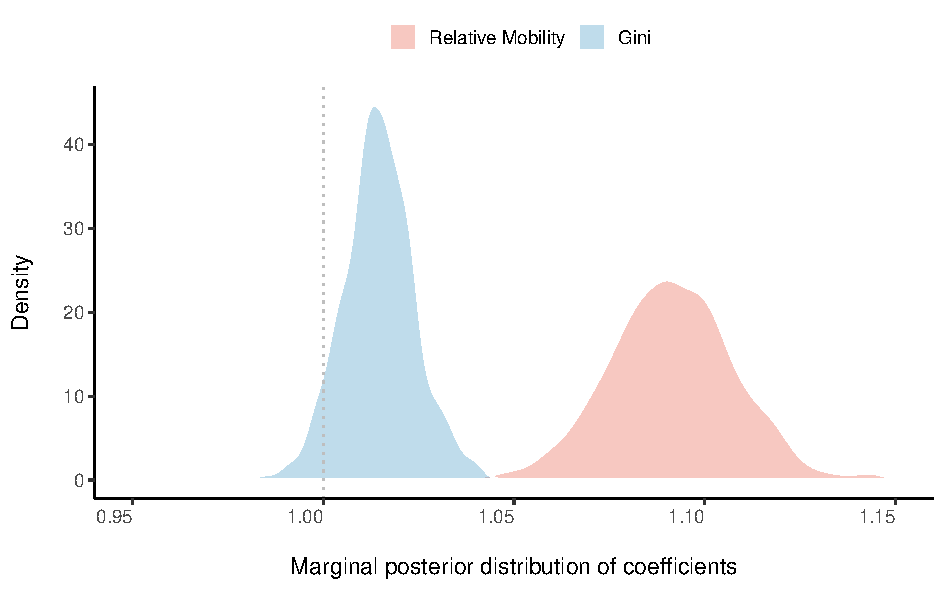
\includegraphics[width=1\textwidth]{figures/files/w4_coefficients_age_pcprior_1_10.pdf}
  \end{subfigure}%

 \begin{subfigure}[b]{.60\linewidth}
   \caption{Men}
    \centering
    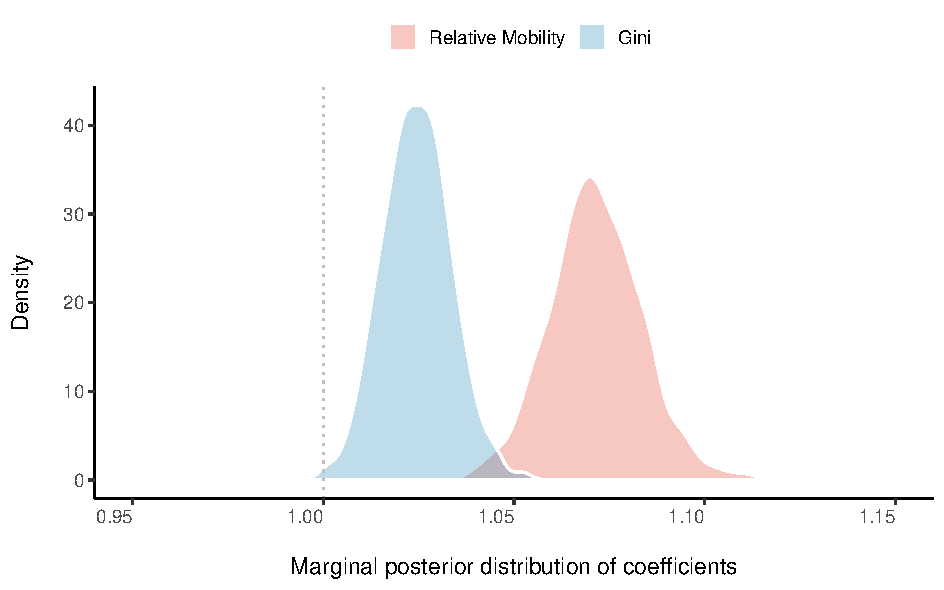
\includegraphics[width=1\textwidth]{figures/files/m4_coefficients_age_pcprior_1_10.pdf}
  \end{subfigure}%
  \label{fig:coefficients_pcprior_1_10}
\end{figure}


\newpage
\begin{figure}[htp]
\caption{95\% Credibility Interval Posterior Distribution of \newline $exp(\beta_m)$ and $exp(\beta_g)$ (Equation \ref{eq:model_age}) by Age Group  \newline Model \textit{Covariates} in Tables \ref{tbl:w_age_pcprior_1_10} and \ref{tbl:m_age_pcprior_1_10}}
\centering

  \begin{subfigure}[b]{.60\linewidth}
    \centering
       \caption{Women}
    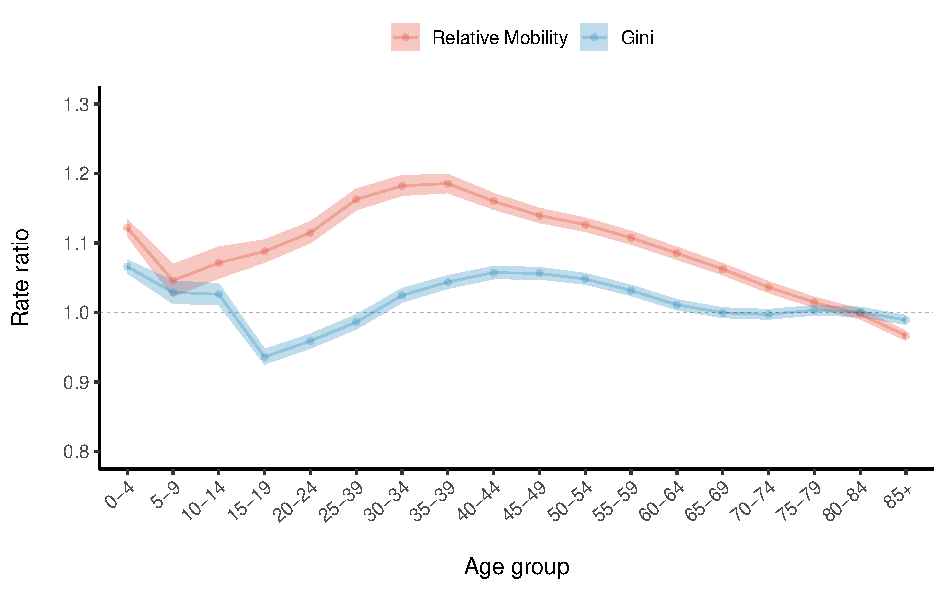
\includegraphics[width=1\textwidth]{figures/files/w4_effects_age_pcprior_1_10.pdf}
  \end{subfigure}%

 \begin{subfigure}[b]{.60\linewidth}
   \caption{Men}
    \centering
    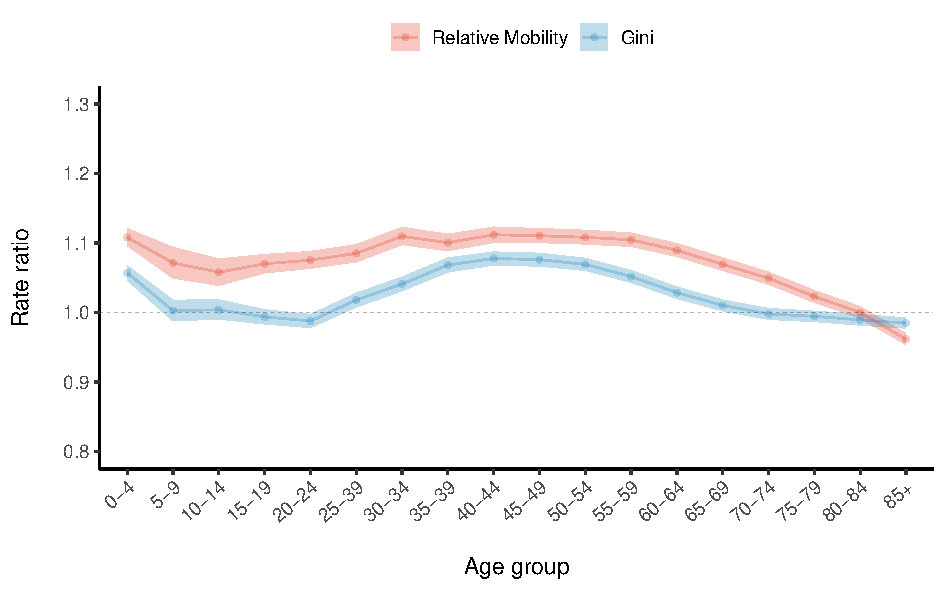
\includegraphics[width=1\textwidth]{figures/files/m4_effects_age_pcprior_1_10.pdf}
  \end{subfigure}%
  \label{fig:effects_age}
\end{figure}


\newpage
\begin{figure}[htp]
\caption{95\% Credibility Interval of Predicted LE Differences 
\newline by Age Group, Increase in One Standard Deviation
\newline Model \textit{Covariates}  in Tables \ref{tbl:w_age_pcprior_1_10_abs} and \ref{tbl:m_age_pcprior_1_10}}
\centering

  \begin{subfigure}[b]{.60\linewidth}
    \centering
       \caption{Women}
    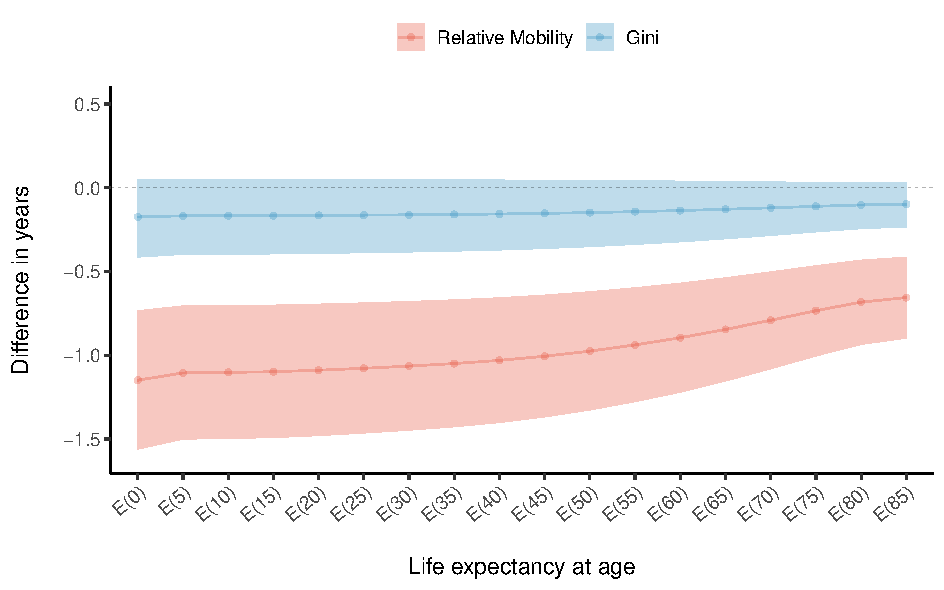
\includegraphics[width=1\textwidth]{figures/files/w4_le_differences_pcprior_1_10.pdf}
  \end{subfigure}%

 \begin{subfigure}[b]{.60\linewidth}
   \caption{Men}
    \centering
    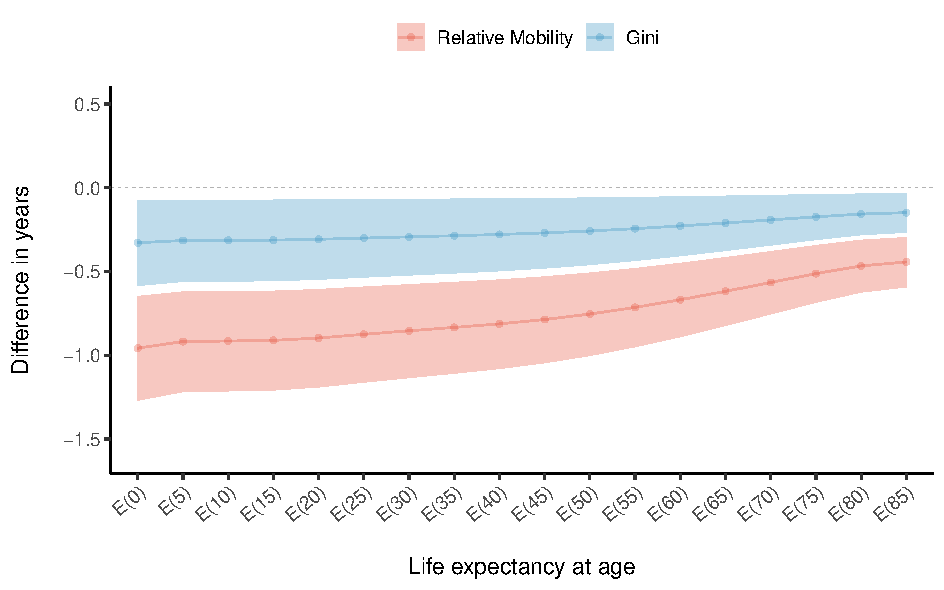
\includegraphics[width=1\textwidth]{figures/files/m4_le_differences_pcprior_1_10.pdf}
  \end{subfigure}%
  \label{fig:le_differences}
\end{figure}


\newpage
\begin{figure}[htp]
\caption{95\% Credibility Interval of Predicted Relative LE Differences 
\newline by Age Group, Increase in One Standard Deviation
\newline Model \textit{Covariates}  in Tables \ref{tbl:w_age_pcprior_1_10_abs} and \ref{tbl:m_age_pcprior_1_10}}
\centering

  \begin{subfigure}[b]{.60\linewidth}
    \centering
       \caption{Women}
    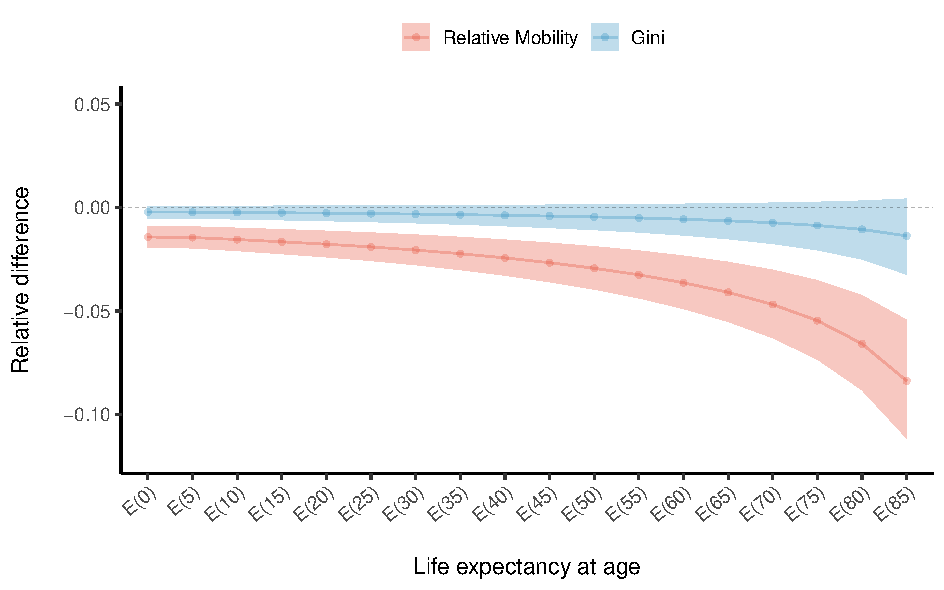
\includegraphics[width=1\textwidth]{figures/files/w4_le_re_differences_pcprior_1_10.pdf}
  \end{subfigure}%

 \begin{subfigure}[b]{.60\linewidth}
   \caption{Men}
    \centering
    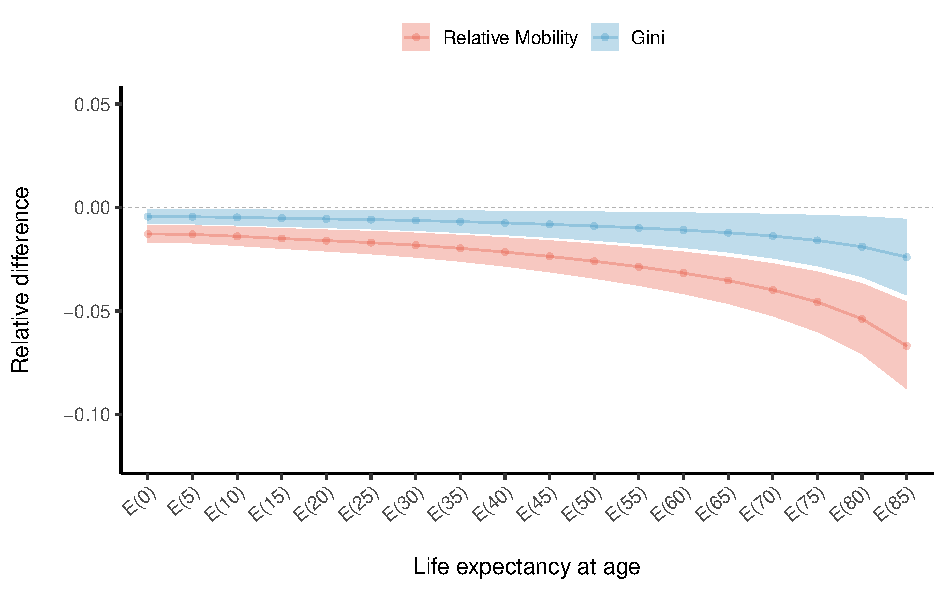
\includegraphics[width=1\textwidth]{figures/files/m4_le_re_differences_pcprior_1_10.pdf}
  \end{subfigure}%
  \label{fig:le_re_differences}
\end{figure}


\newpage
\begin{figure}[htp]
\caption{Posterior Distribution $exp(\beta_{\text{Mob}})$ and $exp(\beta_{\text{Gini}})$ (Equation \ref{eq:model_age}) \newline by Race/Ethnicity and Gender}
\centering

  \begin{subfigure}[b]{.80\linewidth}
    \centering
       \caption{Women}
    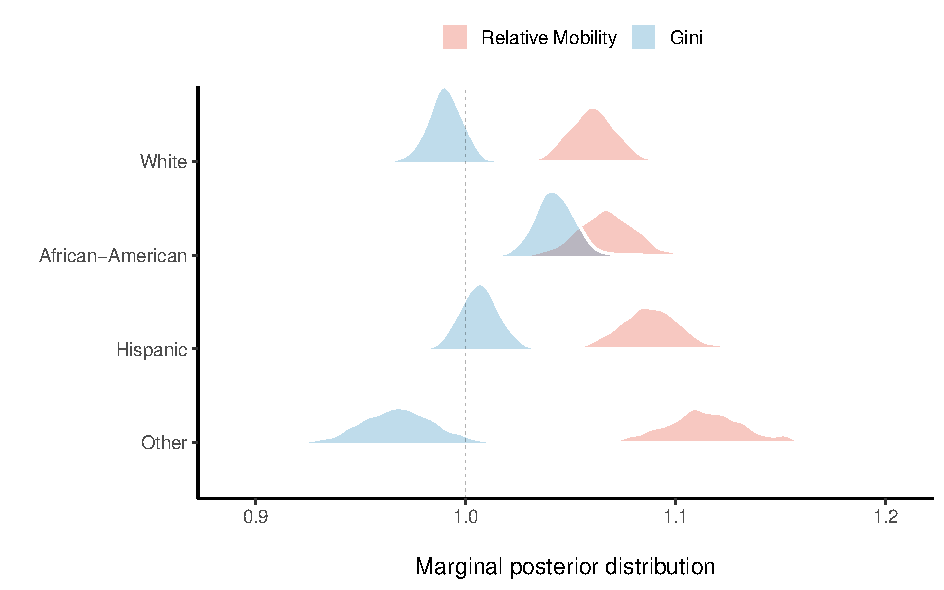
\includegraphics[width=1\textwidth]{figures/files/w_race_dist_pcprior_1_10.pdf}
  \end{subfigure}%

 \begin{subfigure}[b]{.80\linewidth}
   \caption{Men}
    \centering
    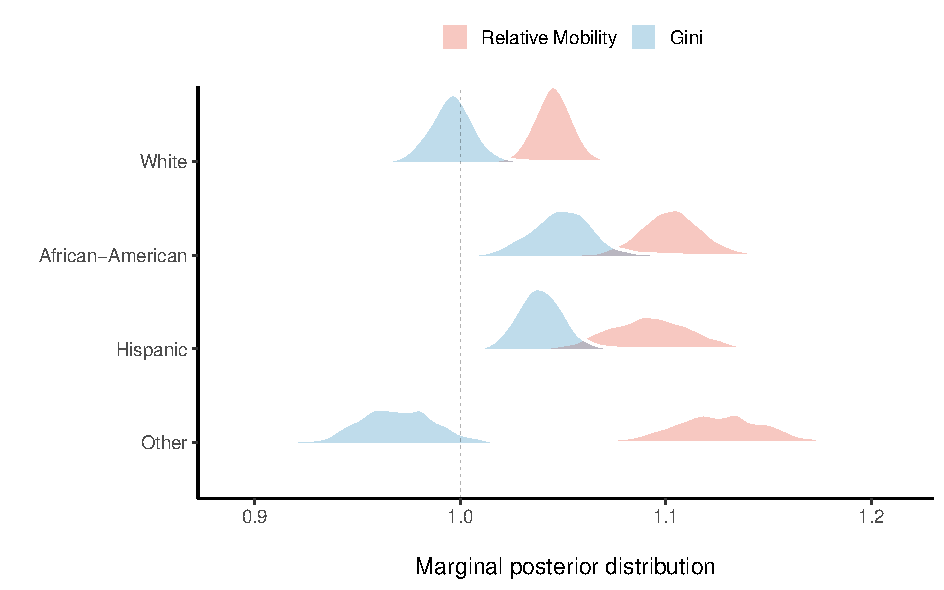
\includegraphics[width=1\textwidth]{figures/files/m_race_dist_pcprior_1_10.pdf}
  \end{subfigure}%
  \label{fig:race}
\end{figure}

\newpage
\begin{figure}[htp]
\caption{95\% Credibility Interval of Predicted LE Differences  \newline 
 by Age Group and Race/Ethnicity, Increase in One Standard Deviation}
\centering

  \begin{subfigure}[b]{.45\linewidth}
    \centering
       \caption{Women - Relative Mobility}
    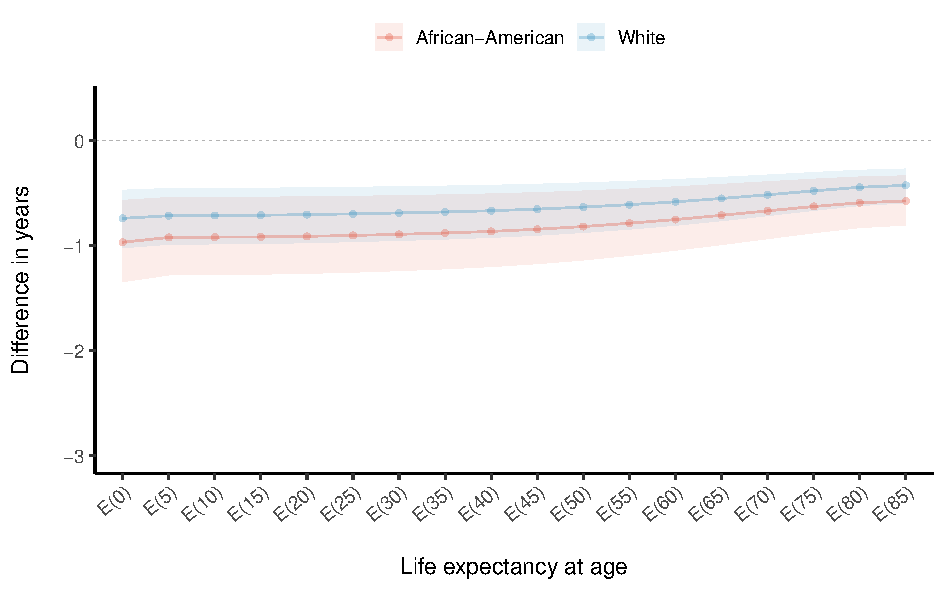
\includegraphics[width=1\textwidth]{figures/files/w_le_differences_race_mob_pcprior_1_10.pdf}%
    ~
  \end{subfigure}
  \begin{subfigure}[b]{.45\linewidth}
    \centering
       \caption{Men - Relative Mobility}
    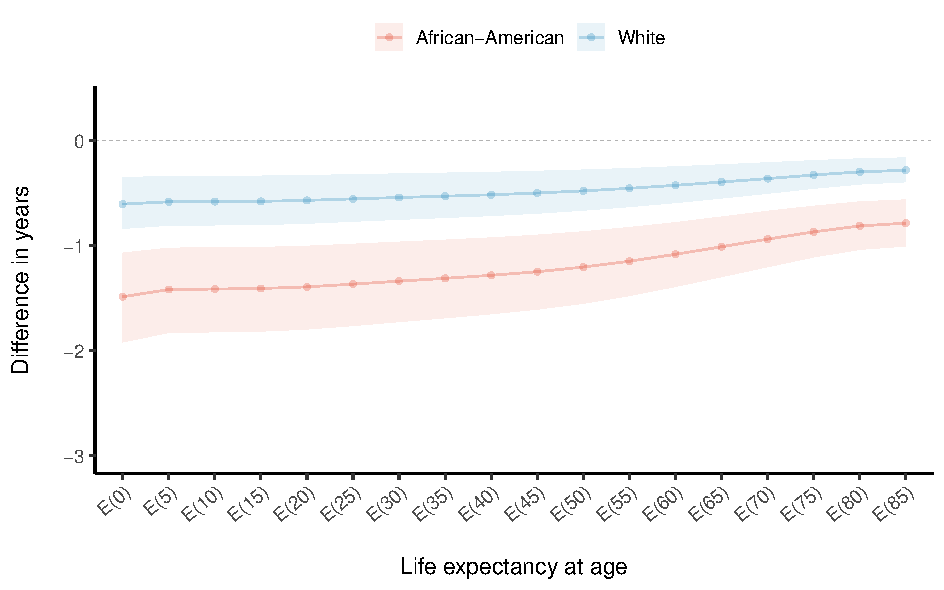
\includegraphics[width=1\textwidth]{figures/files/m_le_differences_race_mob_pcprior_1_10.pdf}
  \end{subfigure}%
  
  \begin{subfigure}[b]{.45\linewidth}
    \centering
       \caption{Women - Gini}
    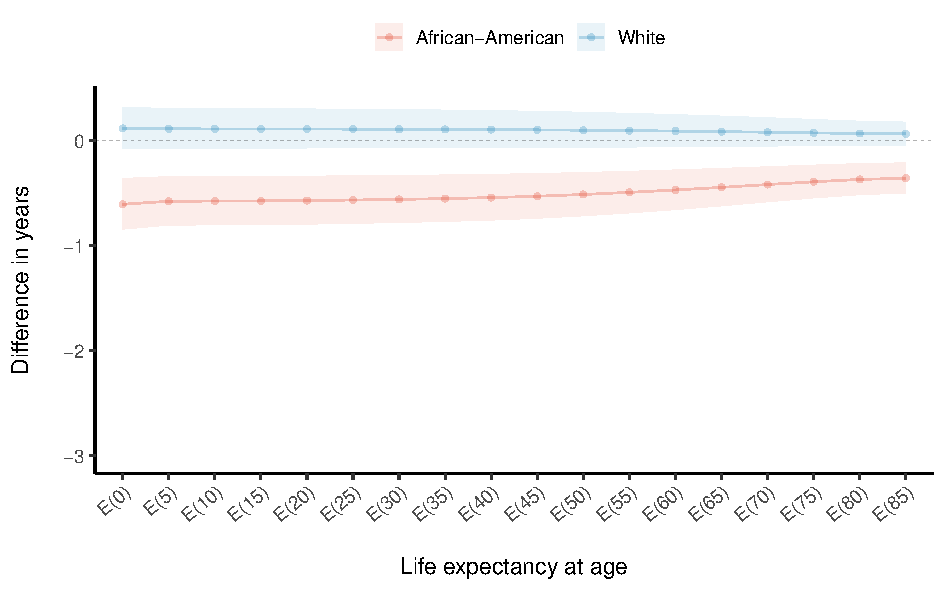
\includegraphics[width=1\textwidth]{figures/files/w_le_differences_race_gini_pcprior_1_10.pdf}
  \end{subfigure}
  \begin{subfigure}[b]{.45\linewidth}
    \centering
       \caption{Men - Gini}
    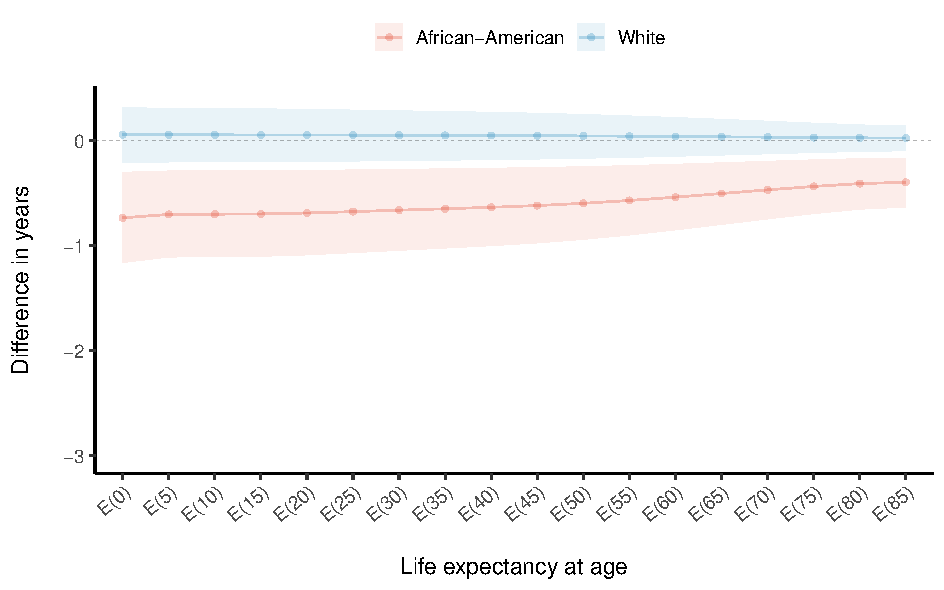
\includegraphics[width=1\textwidth]{figures/files/m_le_differences_race_gini_pcprior_1_10.pdf}
  \end{subfigure}%
  \label{fig:le_differences_age_race}
\end{figure}

\newpage
\begin{figure}[htp]
\caption{95\% Credibility Interval of Predicted LE Relative Differences  \newline 
 by Age Group and Race/Ethnicity, Increase in One Standard Deviation}
\centering

  \begin{subfigure}[b]{.45\linewidth}
    \centering
       \caption{Women - Relative Mobility}
    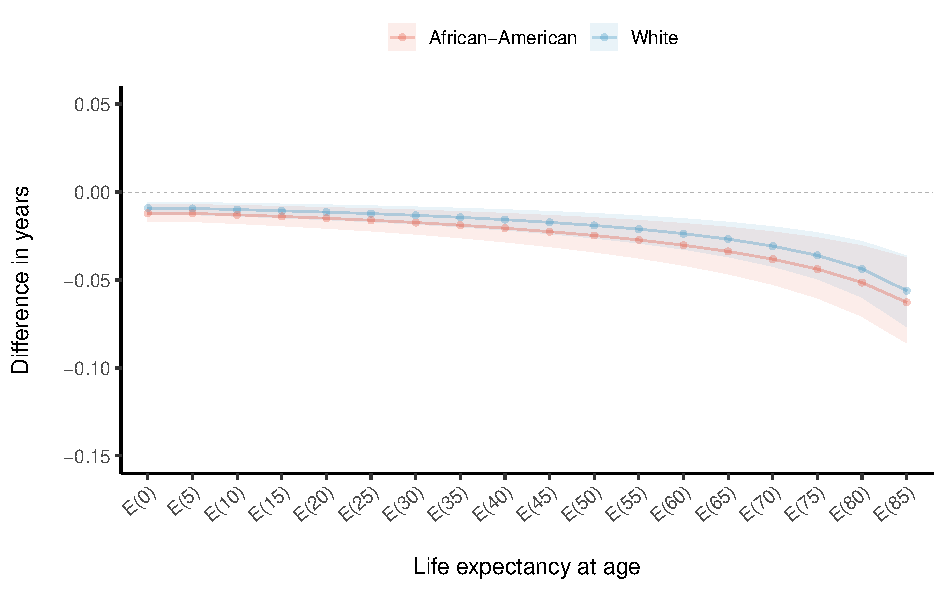
\includegraphics[width=1\textwidth]{figures/files/w_le_re_differences_race_mob_pcprior_1_10.pdf}%
    ~
  \end{subfigure}
  \begin{subfigure}[b]{.45\linewidth}
    \centering
       \caption{Men - Relative Mobility}
    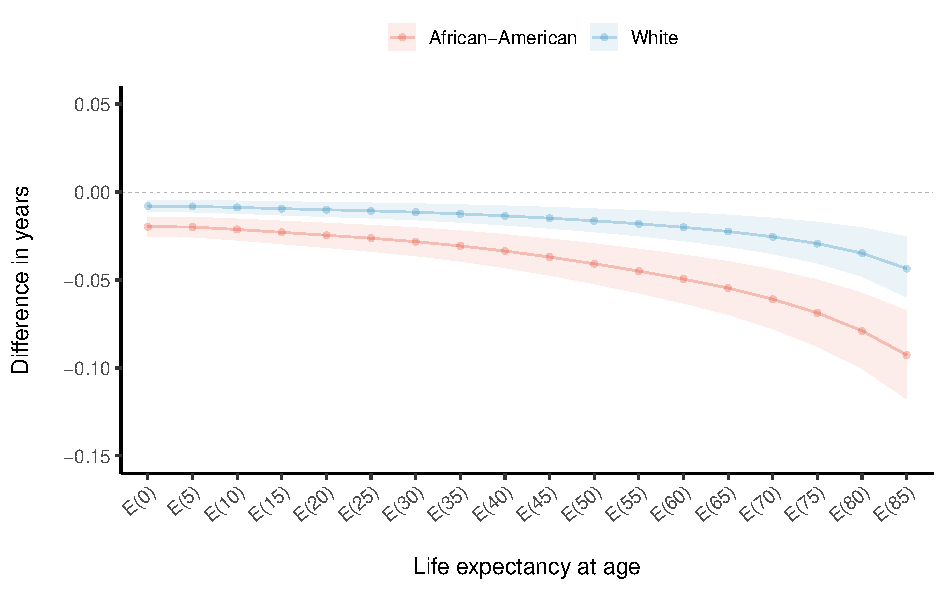
\includegraphics[width=1\textwidth]{figures/files/m_le_re_differences_race_mob_pcprior_1_10.pdf}
  \end{subfigure}%
  
  \begin{subfigure}[b]{.45\linewidth}
    \centering
       \caption{Women - Gini}
    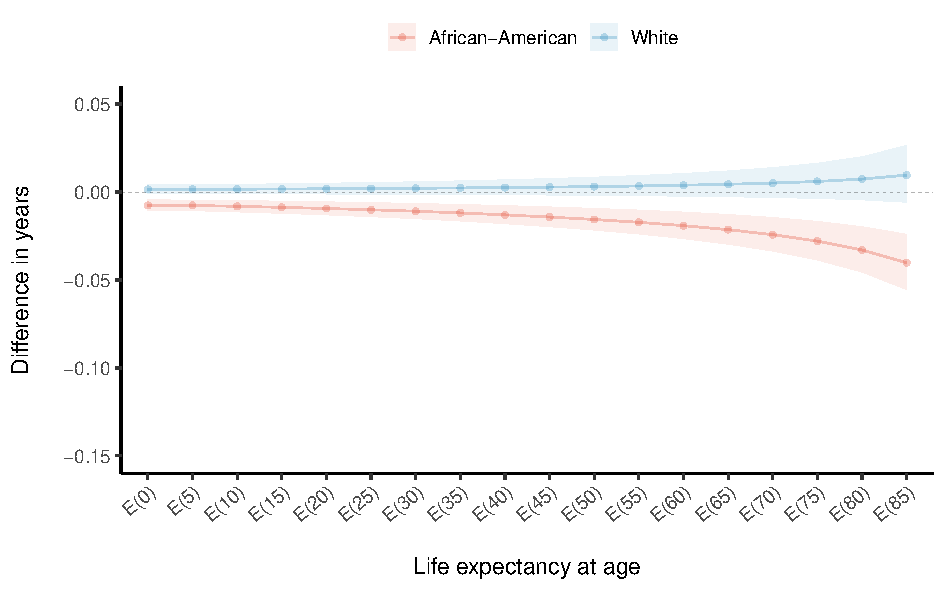
\includegraphics[width=1\textwidth]{figures/files/w_le_re_differences_race_gini_pcprior_1_10.pdf}
  \end{subfigure}
  \begin{subfigure}[b]{.45\linewidth}
    \centering
       \caption{Men - Gini}
    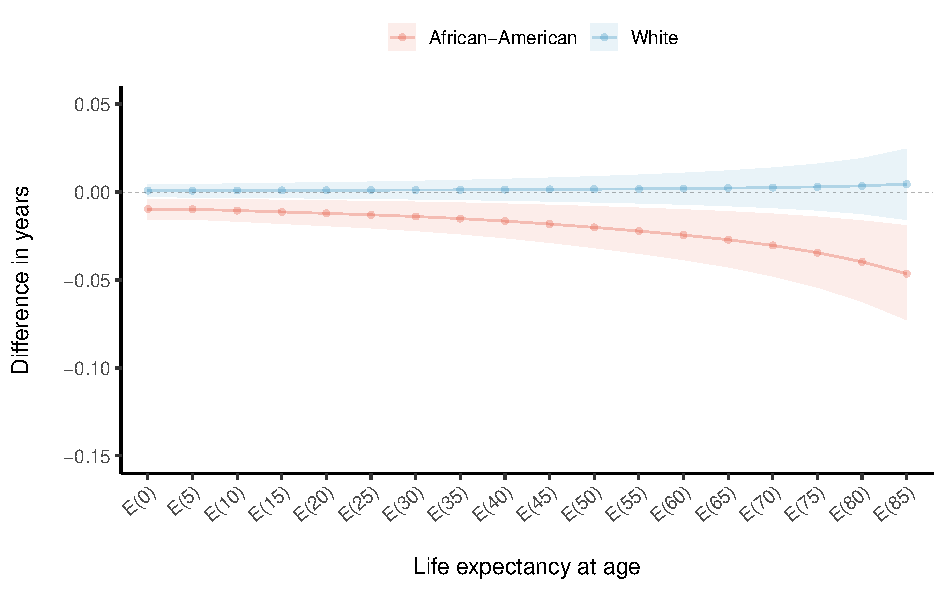
\includegraphics[width=1\textwidth]{figures/files/m_le_re_differences_race_gini_pcprior_1_10.pdf}
  \end{subfigure}%
  \label{fig:le_re_differences_age_race}
\end{figure}

\newpage
\begin{figure}[htp]
\caption{Posterior Distribution $exp(\beta_{\text{Mob}})$ and $exp(\beta{\text{Gini}})$ \newline by Cause of Death and Gender}
\centering

  \begin{subfigure}[b]{.80\linewidth}
    \centering
       \caption{Women}
    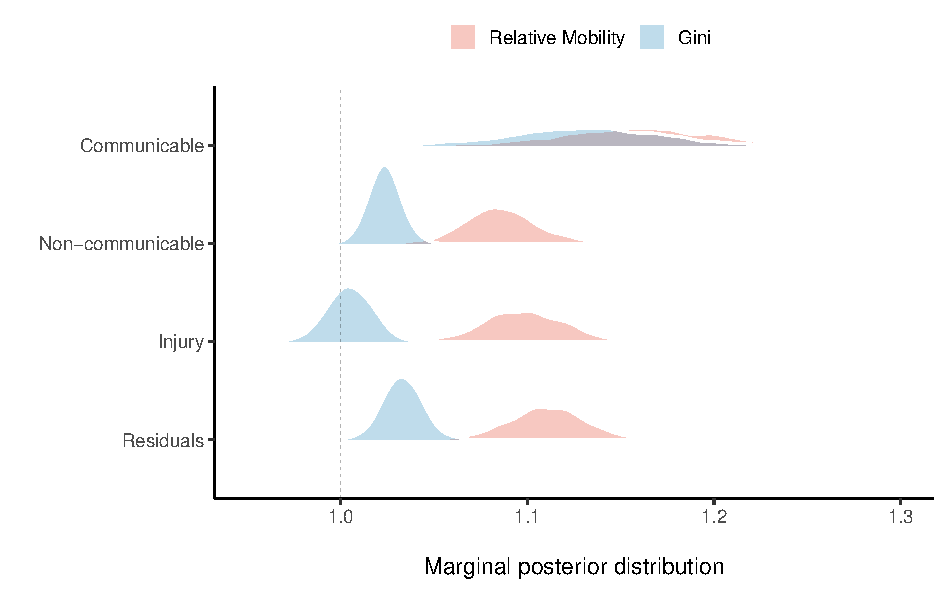
\includegraphics[width=1\textwidth]{figures/files/w_cause_dist_pcprior_1_10.pdf}
  \end{subfigure}%

 \begin{subfigure}[b]{.80\linewidth}
   \caption{Men}
    \centering
    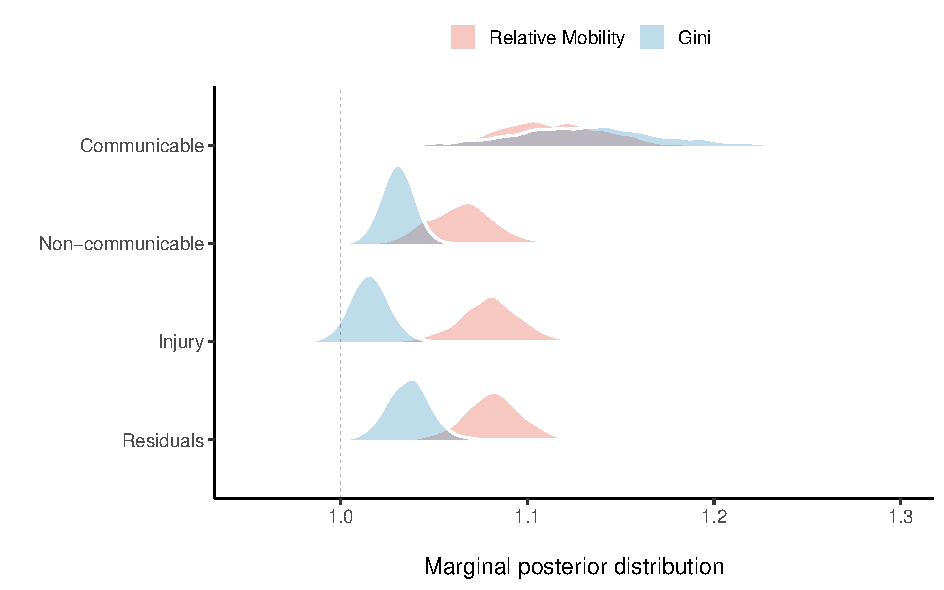
\includegraphics[width=1\textwidth]{figures/files/m_cause_dist_pcprior_1_10.pdf}
  \end{subfigure}%
  \label{fig:cause_of_death}
\end{figure}


% \newpage
% \begin{figure}[htp]
\caption{Posterior Distribution $exp(\beta_{\text{Mob}})$ and $exp(\beta_{\text{Gini}})$ (Equation \ref{eq:model_age}) \newline by Race/Ethnicity and Gender}
\centering

  \begin{subfigure}[b]{.80\linewidth}
    \centering
       \caption{Women}
    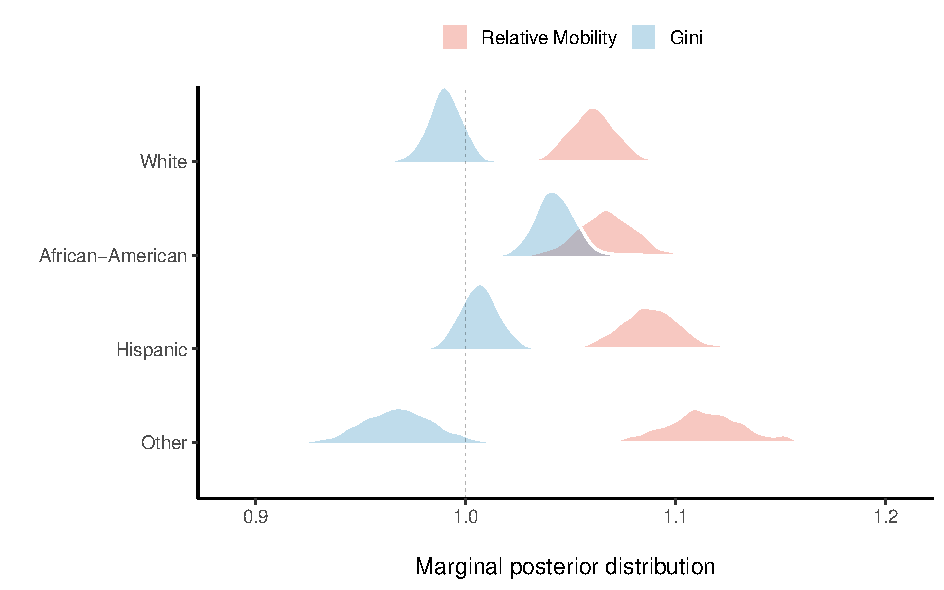
\includegraphics[width=1\textwidth]{figures/files/w_race_dist_pcprior_1_10.pdf}
  \end{subfigure}%

 \begin{subfigure}[b]{.80\linewidth}
   \caption{Men}
    \centering
    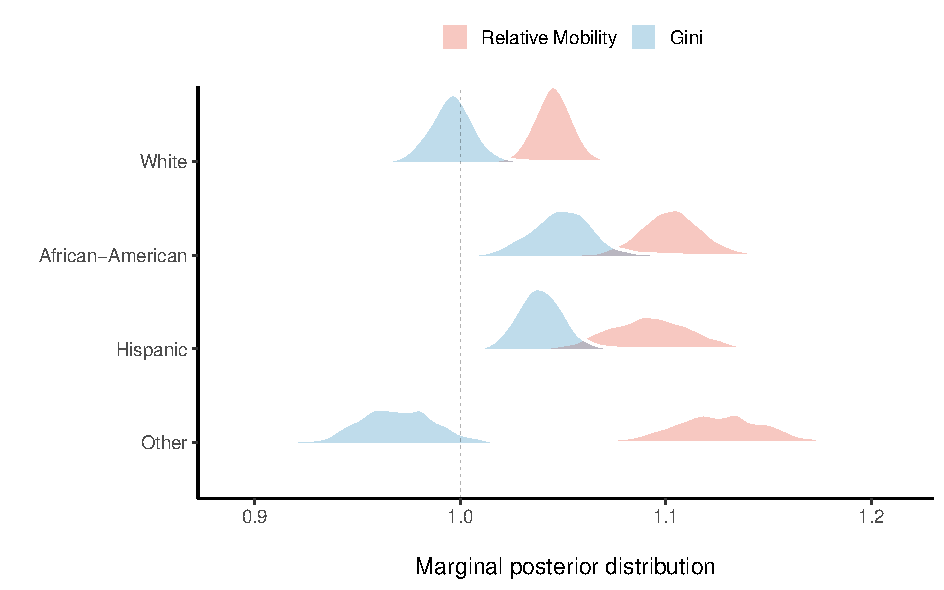
\includegraphics[width=1\textwidth]{figures/files/m_race_dist_pcprior_1_10.pdf}
  \end{subfigure}%
  \label{fig:race}
\end{figure}
% \input{tables/mob_gini_county}
% \input{tables/mob_le_gender_quartile}
% \input{tables/contrast_hipd.tex}
% \input{tables/men_inla_cdc.tex}
% \input{tables/women_inla_cdc.tex}
% \input{tables/contrast_inla_cdc.tex}
% \input{tables/mob_gini_age.tex}
% \input{tables/mob_gini_race.tex}
% \input{tables/mob_gini_cause.tex}



%TC:ignore
%%%%%%%%%%%%%%%%%%%%%%%%%%%%%%%%%%%%%%%%%%%%%%%%%%%%%%%%%%

\clearpage
\singlespacing
\setlength\parskip{12pt}
\bibliographystyle{apa}
\bibliography{ch02}

% \input{tables_figures.tex}

\newpage
\setcounter{page}{1}

\setcounter{section}{0}
\setcounter{table}{0}
\renewcommand{\thetable}{S\arabic{table}}

\setcounter{figure}{0}
\renewcommand{\thefigure}{S\arabic{figure}}

\renewcommand{\thesection}{}
\renewcommand{\thesubsection}{\arabic{section}.\arabic{subsection}}
\makeatletter
\def\@seccntformat#1{\csname #1ignore\expandafter\endcsname\csname the#1\endcsname\quad}
\let\sectionignore\@gobbletwo
\let\latex@numberline\numberline
\def\numberline#1{\if\relax#1\relax\else\latex@numberline{#1}\fi}
\makeatother

\setcounter{section}{0}
\section{Methodological Supplement}\label{sec:appendix}

The code used to create the database and run the models and plots is available at: 

\url{https://github.com/sdaza/dissertation/tree/master/cdc_mortality/notebooks}. 

\subsection{Descriptive Statistics County Level}



\begin{figure}[htp]
\caption{County Coverage Income Mobility Measures (Colored) \newline 2867 counties (91\%)}
\centering

    \includegraphics[width=1\textwidth]{figures/files/coverage_county.pdf}


  \label{fig:county_coverage}
\end{figure}


\newpage
% latex table generated in R 3.5.2 by xtable 1.8-3 package
% Fri Mar 15 16:23:16 2019
\begin{table}[htp]
\centering
\caption{Mean and Standard Deviation of Outcome and Covariates \newline by Relative Income Mobility (IRM), N = 1508 counties} 
\label{tab:descriptives}
\begingroup\scriptsize
\begin{tabular}{lrrrrrr}
  \hline
\addlinespace
& \multicolumn{2}{c}{Full Sample} & \multicolumn{2}{c}{Lowest Quartile IRM} & \multicolumn{2}{c}{Highest Quartile IRM}  \\
Variable & \multicolumn{1}{c}{Mean} & \multicolumn{1}{c}{SD} & \multicolumn{1}{c}{Mean} & \multicolumn{1}{c}{SD} & \multicolumn{1}{c}{Mean} & \multicolumn{1}{c}{SD} \\
\addlinespace
 \hline
  \addlinespace
\multicolumn{7}{l}{\textit{Outcome}} \\
\addlinespace
Age 40 LE Poorest Income Quartile, Women & 41.92 & 1.30 & 41.78 & 1.21 & 42.54 & 1.40 \\ 
  Age 40 LE Richest Income Quartile, Women & 47.43 & 1.65 & 47.13 & 1.59 & 47.84 & 1.62 \\ 
  Age 40 LE Poorest Income Quartile, Men & 36.27 & 1.48 & 35.67 & 1.03 & 37.50 & 1.61 \\ 
  Age 40 LE Richest Income Quartile, Men & 44.83 & 1.75 & 44.35 & 1.73 & 45.50 & 1.73 \\ 
   \addlinespace
\multicolumn{7}{l}{\textit{Covariates}} \\
\addlinespace
Relative Income Mobility (IRM) & -0.27 & 0.07 & -0.35 & 0.04 & -0.17 & 0.03 \\ 
  Gini Coefficient & 0.40 & 0.08 & 0.44 & 0.08 & 0.37 & 0.09 \\ 
  Average Household Income & 34703.83 & 7412.10 & 32164.62 & 5352.69 & 38181.03 & 9498.84 \\ 
  Population & 163432.47 & 397996.80 & 139820.78 & 320852.15 & 234345.21 & 661448.39 \\ 
  Percent Afroamerican & 9.27 & 13.10 & 21.08 & 16.22 & 1.98 & 3.08 \\ 
  Percent Hispanic & 6.36 & 11.54 & 3.97 & 6.57 & 10.36 & 17.58 \\ 
  Crime Rate & 0.01 & 0.00 & 0.01 & 0.00 & 0.01 & 0.00 \\ 
  Income Segregation & 0.04 & 0.03 & 0.04 & 0.03 & 0.05 & 0.03 \\ 
  Unemployment Rate & 0.05 & 0.02 & 0.06 & 0.01 & 0.05 & 0.02 \\ 
  Percent Uninsured & 16.97 & 5.02 & 18.59 & 3.97 & 15.44 & 6.03 \\ 
  Medicare Expenses & 9311.24 & 1407.73 & 9915.20 & 1228.69 & 8365.39 & 1356.87 \\ 
   \addlinespace
\hline
\addlinespace
\end{tabular}
\endgroup
\end{table}


\newpage
\subsection{Goodness of Fit}\label{sec:gof}

We examine the goodness of fit (GOF) of the model \textit{Covariates} in Table \ref{tbl:w_age_pcprior_1_10} and  \ref{tbl:m_age_pcprior_1_10} using the \textit{leave-one-out} predictive measure \textit{probability integral transform} (PIT) \citep{Wang2018}.

The probability integral transform (PIT) is defined as: 

$$PIT_i=p(y^{new}_i\leq y_i|y_{-i})$$

\noindent where $y_{-i}$ denotes the observations $y$ with the $i^{th}$ observation omitted. The only difference between PIT and the posterior predictive p-value is that PIT is computed based on $y_{-i}$ rather than $y$. We would expect PIT statistics to be approximately uniformly distributed for a good model. Values of PIT close to zero or one would indicate observations which are much smaller or larger than expected. One advantage of the PIT relative to other measures such as the \textit{conditional predictive ordinate} (CPO) is that the deviations have a direction.

Figures \ref{fig:pit_loo_pcprior_1_10} and \ref{fig:qqplot_pcprior_1_10} show the histogram and the uniform Q-Q plot of PITs for females and males. As can be seen, the distribution of the PITs is close to a uniform distribution, suggesting that the model reasonably fits the data. 


% \begin{figure}[htp]
\caption{Residuals \newline Model \textit{Covariates} in Tables \ref{tbl:w_age_pcprior_1_10} and \ref{tbl:m_age_pcprior_1_10}}
\centering

  \begin{subfigure}[b]{.50\linewidth}
    \centering
       \caption{Women}
    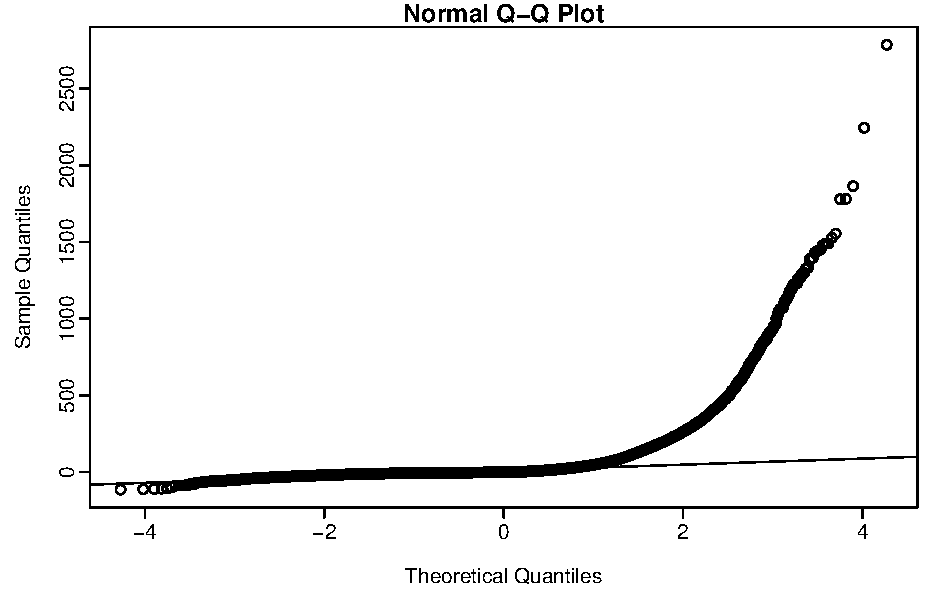
\includegraphics[width=1\textwidth]{figures/files/w4_resid_pcprior_1_10.pdf}
  \end{subfigure}%

 \begin{subfigure}[b]{.50\linewidth}
   \caption{Men}
    \centering
    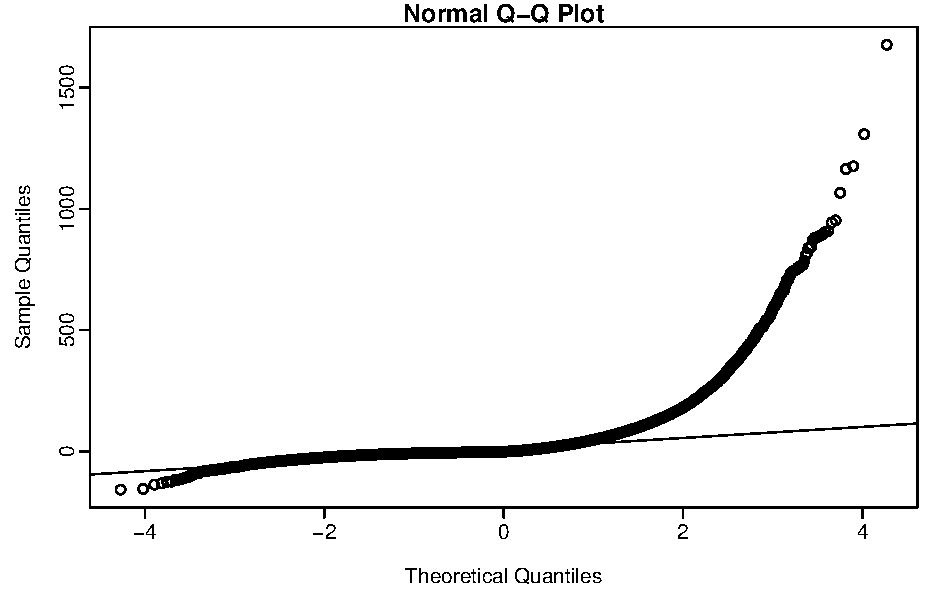
\includegraphics[width=1\textwidth]{figures/files/m4_resid_pcprior_1_10.pdf}
  \end{subfigure}%
  \label{fig:resid_pcprior_1_10}
\end{figure}

\begin{figure}[htp]
\caption{PIT Distribution \newline Model \textit{Covariates} in Tables \ref{tbl:w_age_pcprior_1_10} and \ref{tbl:m_age_pcprior_1_10}}
\centering

  \begin{subfigure}[b]{.50\linewidth}
    \centering
       \caption{Women}
    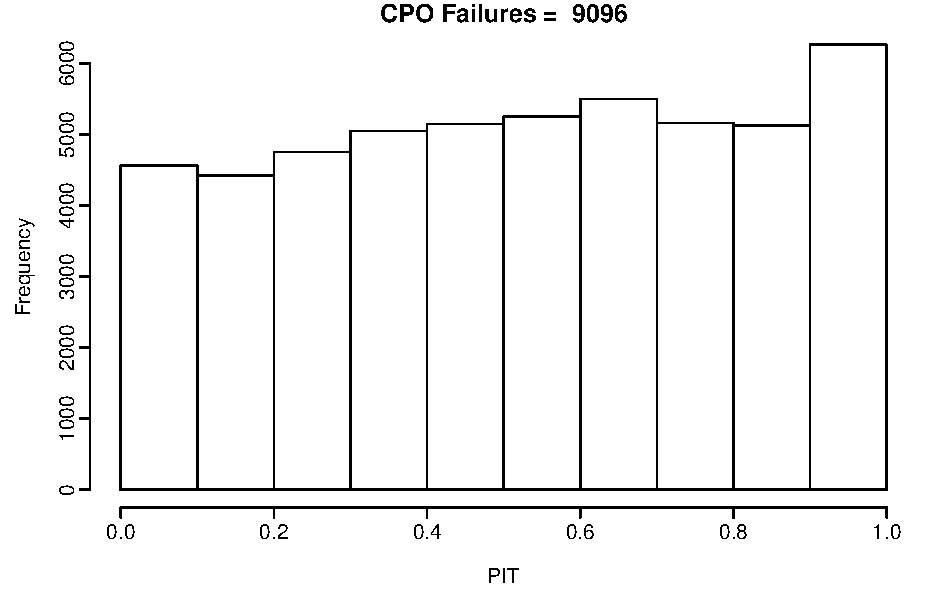
\includegraphics[page=1,width=1\textwidth]{figures/files/w4_loo_pcprior_1_10.pdf}
  \end{subfigure}%

 \begin{subfigure}[b]{.50\linewidth}
   \caption{Men}
    \centering
    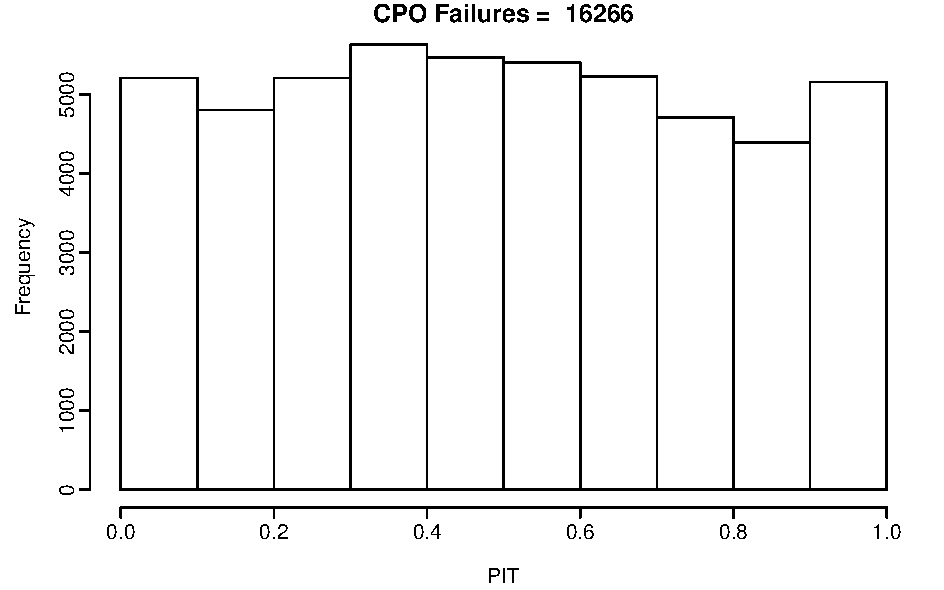
\includegraphics[page=1,width=1\textwidth]{figures/files/m4_loo_pcprior_1_10.pdf}
  \end{subfigure}%
  \label{fig:pit_loo_pcprior_1_10}
\end{figure}


\begin{figure}[htp]
\caption{Q-Q Plot PIT \newline Model \textit{Covariates} in Tables \ref{tbl:w_age_pcprior_1_10} and \ref{tbl:m_age_pcprior_1_10}}
\centering

  \begin{subfigure}[b]{.50\linewidth}
    \centering
       \caption{Women}
    \includegraphics[page=2,width=1\textwidth]{figures/files/w4_loo_pcprior_1_10.pdf}
  \end{subfigure}%

 \begin{subfigure}[b]{.50\linewidth}
   \caption{Men}
    \centering
    \includegraphics[page=2,width=1\textwidth]{figures/files/m4_loo_pcprior_1_10.pdf}
  \end{subfigure}%
  \label{fig:qqplot_pcprior_1_10}
\end{figure}


\newpage
\subsection{Prior sensitivity analysis}\label{sec:sensitivity}


We perform prior sensitivity analysis. We start using the \texttt{R-INLA} default priors. \texttt{R-INLA} uses a precision measure for the variance of the posterior distribution parameters defined as $\tau_{\varepsilon} = \frac{1}{ \sigma^2_{\varepsilon} }$. The default prior distribution for a fixed parameter is a normal distribution with mean 0 and precision $\tau = 0.001$, that is equivalent to $\sigma = 31.62$. We use this diffuse prior  for all fixed regression parameters, except for the intercept in which case the precision is 0, that is, the corresponding sigma is large. For parameterization of random effects \texttt{R-INLA} uses a log gamma distribution for the priors of $log(\tau)$ with shape $a = 1$ and inverse scale $b = 0.00005$. Then, we explore different specifications for Penalized Complexity (PC) priors which are designed to be weakly informative (for more details see \cite{Simpson2017}). PC priors require we specify some scaling. To calibrate the scaling of the random effects prior, we set $U$ and $p$ to different values so that $Pr(\sigma_u > U) < p$. The values we use for $U$ and $p$, respectively, are PC(1,.10), PC(10, .10), PC(10, .0.1). In the first case, for instance, we calibrate the prior so that probability that the standard deviation of the random effect is greater than 1 is lower than .10. 

Table \ref{tbl:w_age_prior_sensitivity} and \ref{tbl:m_age_prior_sensitivity} show the results using different priors with a model equivalent to the \textit{Covariates} model in Table \ref{tbl:w_age_pcprior_1_10} and \ref{tbl:m_age_pcprior_1_10} of the main paper. As can be seen, fixed effects practically do not change when using different prior specifications. The precision of random terms, as expected, shows more variability although changes are small. We decide to use the model with better DIC and WAIC across genders, that is, PC(1, 0.10). 


\begin{table}[htp]
\caption{County Level Poisson Models, Prior Sensitivity, Women, CDC 2000-2014}
\begin{center}
\scalebox{0.65}{
\begin{tabular}{l D{.}{.}{6.11} D{.}{.}{6.11} D{.}{.}{6.11} D{.}{.}{6.11} }
\toprule
 & \multicolumn{1}{c}{INLA Default} & \multicolumn{1}{c}{PC(1, .10)} & \multicolumn{1}{c}{PC(10, .10)} & \multicolumn{1}{c}{PC(10, 0.01)} \\
\midrule
Constant                 & -5.82           & -5.82           & -5.82           & -5.82           \\
                         & [-6.76;\ -4.89] & [-6.70;\ -4.94] & [-6.81;\ -4.83] & [-6.80;\ -4.84] \\
Income relative mobility & 0.09            & 0.09            & 0.09            & 0.09            \\
                         & [0.06;\ 0.11]   & [0.06;\ 0.12]   & [0.06;\ 0.12]   & [0.06;\ 0.12]   \\
Gini                     & 0.01            & 0.01            & 0.01            & 0.01            \\
                         & [-0.00;\ 0.03]  & [-0.00;\ 0.03]  & [-0.00;\ 0.03]  & [-0.00;\ 0.03]  \\
Random Effects           &                 &                 &                 &                 \\
                         &                 &                 &                 &                 \\
\quad SD observations    & 0.10            & 0.10            & 0.10            & 0.10            \\
                         & [0.10;\ 0.10]   & [0.10;\ 0.10]   & [0.10;\ 0.10]   & [0.10;\ 0.10]   \\
\quad SD age group       & 2.00            & 1.90            & 2.14            & 2.10            \\
                         & [1.43;\ 2.73]   & [1.43;\ 2.67]   & [1.53;\ 3.10]   & [1.51;\ 3.01]   \\
\quad SD counties        & 0.09            & 0.09            & 0.09            & 0.09            \\
                         & [0.09;\ 0.09]   & [0.09;\ 0.09]   & [0.09;\ 0.09]   & [0.08;\ 0.09]   \\
\quad SD states          & 0.06            & 0.06            & 0.06            & 0.06            \\
                         & [0.05;\ 0.08]   & [0.05;\ 0.08]   & [0.05;\ 0.08]   & [0.05;\ 0.08]   \\
\quad SD mobility by age & 0.06            & 0.06            & 0.06            & 0.07            \\
                         & [0.04;\ 0.08]   & [0.04;\ 0.09]   & [0.05;\ 0.09]   & [0.05;\ 0.09]   \\
\quad SD gini by age     & 0.03            & 0.04            & 0.04            & 0.04            \\
                         & [0.02;\ 0.05]   & [0.03;\ 0.05]   & [0.03;\ 0.05]   & [0.03;\ 0.05]   \\
\midrule
DIC                      & 364144          & 364144          & 364142          & 364134          \\
WAIC                     & 362517          & 362521          & 362514          & 362506          \\
\bottomrule
\multicolumn{5}{l}{\scriptsize{Note: Selected coefficients (mean of marginal posterior distribution).
       Poisson model with offset = \texttt{log(population)}. 95\% credibility intervals.}}
\end{tabular}
}
\label{tbl:w_age_prior_sensitivity}
\end{center}
\end{table}


\begin{table}[htp]
\caption{County Level Poisson Models, Prior Sensitivity, Men, CDC 2000-2014}
\begin{center}
\scalebox{0.65}{
\begin{tabular}{l D{.}{.}{6.11} D{.}{.}{6.11} D{.}{.}{6.11} D{.}{.}{6.11} }
\toprule
 & \multicolumn{1}{c}{INLA Default} & \multicolumn{1}{c}{PC(1, .10)} & \multicolumn{1}{c}{PC(10, .10)} & \multicolumn{1}{c}{PC(10, 0.01)} \\
\midrule
Constant                 & -5.31           & -5.31           & -5.31           & -5.31           \\
                         & [-6.22;\ -4.41] & [-6.17;\ -4.45] & [-6.26;\ -4.36] & [-6.23;\ -4.39] \\
Income relative mobility & 0.07            & 0.07            & 0.07            & 0.07            \\
                         & [0.05;\ 0.09]   & [0.05;\ 0.09]   & [0.05;\ 0.09]   & [0.05;\ 0.09]   \\
Gini                     & 0.02            & 0.02            & 0.02            & 0.02            \\
                         & [0.01;\ 0.04]   & [0.01;\ 0.04]   & [0.01;\ 0.04]   & [0.01;\ 0.04]   \\
Random Effects           &                 &                 &                 &                 \\
                         &                 &                 &                 &                 \\
\quad SD observations    & 0.12            & 0.12            & 0.12            & 0.13            \\
                         & [0.12;\ 0.13]   & [0.12;\ 0.13]   & [0.12;\ 0.13]   & [0.12;\ 0.13]   \\
\quad SD age group       & 1.90            & 1.85            & 2.04            & 2.00            \\
                         & [1.28;\ 2.57]   & [1.35;\ 2.43]   & [1.47;\ 2.99]   & [1.44;\ 2.81]   \\
\quad SD counties        & 0.10            & 0.10            & 0.10            & 0.10            \\
                         & [0.10;\ 0.11]   & [0.10;\ 0.11]   & [0.10;\ 0.11]   & [0.10;\ 0.10]   \\
\quad SD states          & 0.06            & 0.06            & 0.06            & 0.06            \\
                         & [0.04;\ 0.07]   & [0.05;\ 0.08]   & [0.05;\ 0.08]   & [0.05;\ 0.08]   \\
\quad SD mobility by age & 0.04            & 0.04            & 0.05            & 0.04            \\
                         & [0.03;\ 0.06]   & [0.03;\ 0.06]   & [0.03;\ 0.06]   & [0.03;\ 0.06]   \\
\quad SD gini by age     & 0.03            & 0.04            & 0.04            & 0.04            \\
                         & [0.02;\ 0.05]   & [0.03;\ 0.05]   & [0.03;\ 0.05]   & [0.03;\ 0.05]   \\
\midrule
DIC                      & 394915          & 394906          & 394913          & 394900          \\
WAIC                     & 392796          & 392766          & 392791          & 392742          \\
\bottomrule
\multicolumn{5}{l}{\scriptsize{Note: Selected coefficients (mean of marginal posterior distribution).
            Poisson model with offset = \texttt{log(population)}. 95\% credibility intervals.}}
\end{tabular}
}
\label{tbl:m_age_prior_sensitivity}
\end{center}
\end{table}



\clearpage
\subsection{Results Using Absolute Mobility}

We run of the models of the paper using an absolute upward mobility score or ``the mean rank (in the national income distribution) of children whose parents are at the 25\textsuperscript{th} percentile of the national parent income distribution'' \citep[p. 7]{Chetty2014}.

Although at the national level both the relative and absolute measure of mobility provide similar information, when studying small areas a child's rank in the national income distribution would be an absolute outcome because income in a given areas have little impact on the national distribution. We use a \textit{permanent-resident} version of income mobility measures, that is, parents who stay in the same counties between 1996-2012. Note that children who grow up in a county may have moved out as adults.

Absolute upward income mobility ranges from 0 to 1, and higher values correspond to large income mobility. We multiply the absolute upward mobility score by -1 so that the interpretation and expected association of relative and absolute income mobility were the same (i.e., increases in  income mobility and inequality is expected to rise mortality risk). The results  are similar to the ones using relative income mobility, what is not surprising because the correlation between both measures is high (-0.70). Still, there are some differences is worth to mention. 

IRM and GI ratios by age-group look more similar by gender than when using relative income mobility. The IRM male curve still look smoother than the female one, and the magnitude of the peak is greater for women (see Figure \ref{fig:effects_age_abs}). Life expectancy differences are of the same order of magnitude (one year), but the decrease of differences at older ages is faster among males than females (see Figure \ref{fig:le_differences_abs}). Relative differences are shown in Figure \ref{fig:le_re_differences_abs}. Finally, there is also a much clear difference in the effect of IRM between Non-Hispanic White males and other groups (see Figure \ref{fig:race_abs}).

\begin{figure}[htp]
\caption{Posterior Distribution of $exp(\beta_{\text{Mob}})$ and $exp(\beta_{\text{Gini}})$ by Gender \newline Model \textit{Covariates} in Tables \ref{tbl:w_age_pcprior_1_10_abs} and \ref{tbl:m_age_pcprior_1_10_abs}}
\centering

  \begin{subfigure}[b]{.60\linewidth}
    \centering
       \caption{Women}
    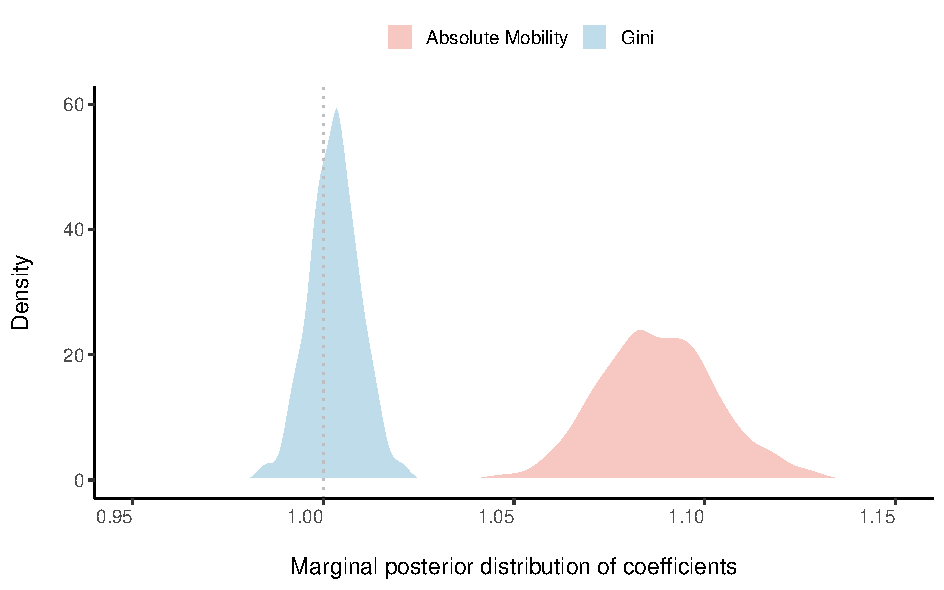
\includegraphics[width=1\textwidth]{figures/files/w4_coefficients_age_pcprior_1_10_abs.pdf}
  \end{subfigure}%

 \begin{subfigure}[b]{.60\linewidth}
   \caption{Men}
    \centering
    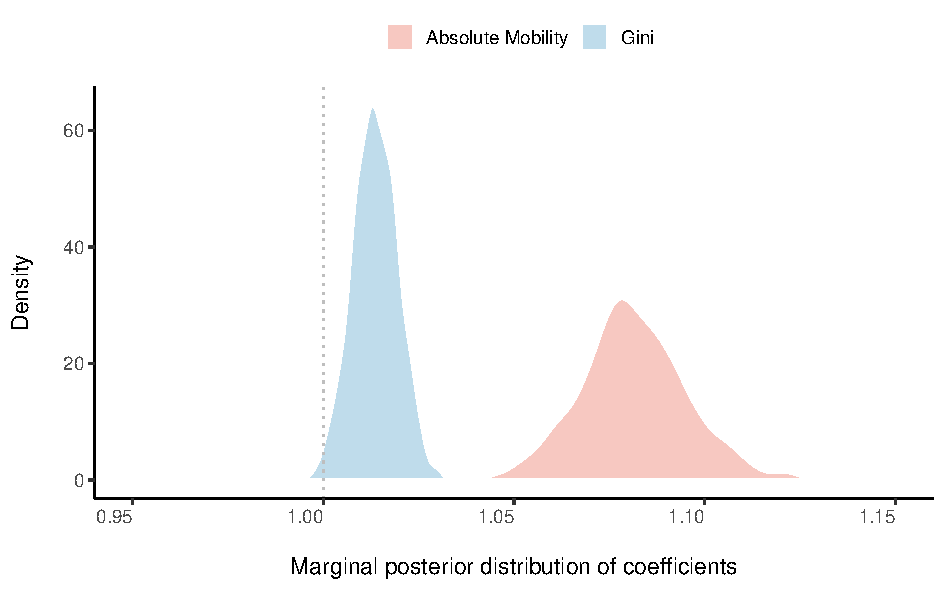
\includegraphics[width=1\textwidth]{figures/files/m4_coefficients_age_pcprior_1_10_abs.pdf}
  \end{subfigure}%
  \label{fig:coefficients_pcprior_1_10_abs}
\end{figure}


\newpage

\begin{sidewaystable}[htp]
\caption{County Level Poisson Models Absolute Mobility \newline PC prior $= Pr(\sigma > 1) < 0.10$, Women, CDC 2000-2014}
\begin{center}
\scalebox{0.65}{
\begin{tabular}{l D{.}{.}{6.11} D{.}{.}{6.11} D{.}{.}{6.11} D{.}{.}{6.11} D{.}{.}{6.11} D{.}{.}{6.11} }
\toprule
 & \multicolumn{1}{c}{Baseline} & \multicolumn{1}{c}{Varying-Coefficient} & \multicolumn{1}{c}{Absolute mobility x Gini} & \multicolumn{1}{c}{Absolute mobility x Income} & \multicolumn{1}{c}{Covariates} & \multicolumn{1}{c}{Spatial} \\
\midrule
Constant                       & -5.81           & -5.83           & -5.82           & -5.82           & -5.82           & -5.82           \\
                               & [-6.71;\ -4.92] & [-6.71;\ -4.94] & [-6.71;\ -4.94] & [-6.71;\ -4.94] & [-6.71;\ -4.94] & [-6.64;\ -4.99] \\
Income absolute mobility       & 0.08            & 0.09            & 0.09            & 0.09            & 0.08            & 0.09            \\
                               & [0.07;\ 0.08]   & [0.06;\ 0.12]   & [0.06;\ 0.12]   & [0.07;\ 0.12]   & [0.05;\ 0.11]   & [0.06;\ 0.11]   \\
Gini                           & 0.00            & -0.00           & 0.00            & -0.00           & 0.00            & 0.01            \\
                               & [-0.00;\ 0.01]  & [-0.01;\ 0.01]  & [-0.01;\ 0.01]  & [-0.01;\ 0.01]  & [-0.01;\ 0.02]  & [-0.01;\ 0.02]  \\
Log income                     & -0.37           & -0.36           & -0.36           & -0.36           & -0.27           & -0.25           \\
                               & [-0.39;\ -0.34] & [-0.39;\ -0.34] & [-0.39;\ -0.34] & [-0.39;\ -0.34] & [-0.30;\ -0.24] & [-0.28;\ -0.22] \\
Absolute mobility x Gini       &                 &                 & -0.00           &                 &                 &                 \\
                               &                 &                 & [-0.00;\ 0.00]  &                 &                 &                 \\
Absolute mobility x Log income &                 &                 &                 & 0.01            &                 &                 \\
                               &                 &                 &                 & [-0.02;\ 0.03]  &                 &                 \\
Random Effects                 &                 &                 &                 &                 &                 &                 \\
                               &                 &                 &                 &                 &                 &                 \\
\quad SD observations          & 0.13            & 0.11            & 0.11            & 0.11            & 0.11            & 0.11            \\
                               & [0.12;\ 0.13]   & [0.11;\ 0.11]   & [0.11;\ 0.11]   & [0.11;\ 0.11]   & [0.11;\ 0.11]   & [0.11;\ 0.11]   \\
\quad SD age group             & 1.92            & 1.92            & 1.88            & 1.91            & 1.91            & 1.85            \\
                               & [1.43;\ 2.57]   & [1.43;\ 2.73]   & [1.41;\ 2.55]   & [1.44;\ 2.55]   & [1.43;\ 2.60]   & [1.43;\ 2.48]   \\
\quad SD counties              & 0.10            & 0.10            & 0.10            & 0.10            & 0.09            & 0.12            \\
                               & [0.10;\ 0.10]   & [0.10;\ 0.10]   & [0.10;\ 0.10]   & [0.10;\ 0.10]   & [0.09;\ 0.10]   & [0.11;\ 0.12]   \\
\quad Phi counties             &                 &                 &                 &                 &                 & 1.16            \\
                               &                 &                 &                 &                 &                 & [1.08;\ 1.39]   \\
\quad SD states                & 0.09            & 0.09            & 0.09            & 0.09            & 0.07            & 0.05            \\
                               & [0.07;\ 0.11]   & [0.06;\ 0.11]   & [0.06;\ 0.11]   & [0.07;\ 0.11]   & [0.05;\ 0.09]   & [0.03;\ 0.06]   \\
\quad SD mobility by age       &                 & 0.06            & 0.06            & 0.06            & 0.06            & 0.06            \\
                               &                 & [0.04;\ 0.09]   & [0.04;\ 0.09]   & [0.04;\ 0.08]   & [0.04;\ 0.08]   & [0.04;\ 0.08]   \\
\quad SD gini by age           &                 & 0.03            & 0.03            & 0.03            & 0.03            & 0.03            \\
                               &                 & [0.02;\ 0.04]   & [0.02;\ 0.04]   & [0.02;\ 0.04]   & [0.02;\ 0.04]   & [0.02;\ 0.05]   \\
\midrule
DIC                            & 368244          & 367192          & 367191          & 367195          & 367108          & 366995          \\
WAIC                           & 365811          & 365279          & 365275          & 365289          & 365156          & 365075          \\
\bottomrule
\multicolumn{7}{l}{\scriptsize{Note: Selected coefficients (mean of marginal posterior distribution).
           Poisson model with offset = \texttt{log(population)}. 95\% credibility intervals.}}
\end{tabular}
}
\label{tbl:w_age_pcprior_1_10_abs}
\end{center}
\end{sidewaystable}


\newpage

\begin{sidewaystable}[htp]
\caption{County Level Poisson Models Absolute Mobility \newline PC Prior $= Pr(\sigma > 1) < 0.10$, Men, CDC 2000-2014}
\begin{center}
\scalebox{0.65}{
\begin{tabular}{l D{.}{.}{6.11} D{.}{.}{6.11} D{.}{.}{6.11} D{.}{.}{6.11} D{.}{.}{6.11} D{.}{.}{6.11} }
\toprule
 & \multicolumn{1}{c}{Baseline} & \multicolumn{1}{c}{Varying-Coefficient} & \multicolumn{1}{c}{Absolute mobility x Gini} & \multicolumn{1}{c}{Absolute mobility x Income} & \multicolumn{1}{c}{Covariates} & \multicolumn{1}{c}{Spatial} \\
\midrule
Constant                       & -5.31           & -5.32           & -5.32           & -5.32           & -5.31           & -5.31           \\
                               & [-6.16;\ -4.46] & [-6.17;\ -4.47] & [-6.17;\ -4.47] & [-6.16;\ -4.47] & [-6.12;\ -4.51] & [-6.18;\ -4.43] \\
Income absolute mobility       & 0.08            & 0.09            & 0.09            & 0.09            & 0.08            & 0.09            \\
                               & [0.07;\ 0.09]   & [0.06;\ 0.11]   & [0.06;\ 0.11]   & [0.06;\ 0.11]   & [0.05;\ 0.10]   & [0.06;\ 0.11]   \\
Gini                           & 0.01            & 0.02            & 0.01            & 0.01            & 0.01            & 0.01            \\
                               & [0.01;\ 0.02]   & [0.00;\ 0.03]   & [0.00;\ 0.02]   & [0.00;\ 0.03]   & [0.00;\ 0.03]   & [0.00;\ 0.03]   \\
Log income                     & -0.35           & -0.35           & -0.36           & -0.36           & -0.21           & -0.16           \\
                               & [-0.38;\ -0.32] & [-0.38;\ -0.32] & [-0.39;\ -0.33] & [-0.39;\ -0.33] & [-0.24;\ -0.18] & [-0.20;\ -0.13] \\
Absolute mobility x Gini       &                 &                 & 0.01            &                 &                 &                 \\
                               &                 &                 & [0.00;\ 0.01]   &                 &                 &                 \\
Absolute mobility x Log income &                 &                 &                 & 0.02            &                 &                 \\
                               &                 &                 &                 & [-0.01;\ 0.04]  &                 &                 \\
Random Effects                 &                 &                 &                 &                 &                 &                 \\
                               &                 &                 &                 &                 &                 &                 \\
\quad SD observations          & 0.14            & 0.13            & 0.13            & 0.13            & 0.13            & 0.13            \\
                               & [0.14;\ 0.14]   & [0.13;\ 0.13]   & [0.13;\ 0.13]   & [0.13;\ 0.13]   & [0.13;\ 0.13]   & [0.13;\ 0.13]   \\
\quad SD age group             & 1.82            & 1.83            & 1.84            & 1.81            & 1.94            & 1.84            \\
                               & [1.37;\ 2.50]   & [1.39;\ 2.46]   & [1.37;\ 2.51]   & [1.37;\ 2.42]   & [1.37;\ 3.03]   & [1.28;\ 2.49]   \\
\quad SD counties              & 0.12            & 0.11            & 0.11            & 0.11            & 0.10            & 0.16            \\
                               & [0.11;\ 0.12]   & [0.11;\ 0.12]   & [0.11;\ 0.12]   & [0.11;\ 0.12]   & [0.09;\ 0.11]   & [0.15;\ 0.17]   \\
\quad Phi counties             &                 &                 &                 &                 &                 & 1.03            \\
                               &                 &                 &                 &                 &                 & [1.01;\ 1.07]   \\
\quad SD states                & 0.09            & 0.08            & 0.08            & 0.08            & 0.07            & 0.06            \\
                               & [0.07;\ 0.11]   & [0.07;\ 0.11]   & [0.07;\ 0.10]   & [0.07;\ 0.10]   & [0.05;\ 0.09]   & [0.04;\ 0.08]   \\
\quad SD mobility by age       &                 & 0.05            & 0.05            & 0.05            & 0.05            & 0.05            \\
                               &                 & [0.04;\ 0.07]   & [0.04;\ 0.07]   & [0.04;\ 0.08]   & [0.04;\ 0.07]   & [0.04;\ 0.08]   \\
\quad SD gini by age           &                 & 0.02            & 0.02            & 0.02            & 0.02            & 0.02            \\
                               &                 & [0.01;\ 0.03]   & [0.02;\ 0.03]   & [0.02;\ 0.03]   & [0.02;\ 0.03]   & [0.02;\ 0.03]   \\
\midrule
DIC                            & 392498          & 391536          & 391534          & 391534          & 391452          & 391387          \\
WAIC                           & 389440          & 389078          & 389078          & 389076          & 388943          & 388923          \\
\bottomrule
\multicolumn{7}{l}{\scriptsize{Note: Selected coefficients (mean of marginal posterior distribution).
       Poisson model with offset = \texttt{log(population)}. 95\% credibility intervals.}}
\end{tabular}
}
\label{tbl:m_age_pcprior_1_10_abs}
\end{center}
\end{sidewaystable}


\clearpage
\begin{figure}[htp]
\caption{95\% Credibility Interval Posterior Distribution of \newline $exp(\beta_m)$ and $exp(\beta_g)$ (see Equation \ref{eq:model_age}) by Age Group  \newline Model \textit{Covariates} in Tables \ref{tbl:w_age_pcprior_1_10_abs} and \ref{tbl:m_age_pcprior_1_10_abs}}
\centering

  \begin{subfigure}[b]{.60\linewidth}
    \centering
       \caption{Women}
    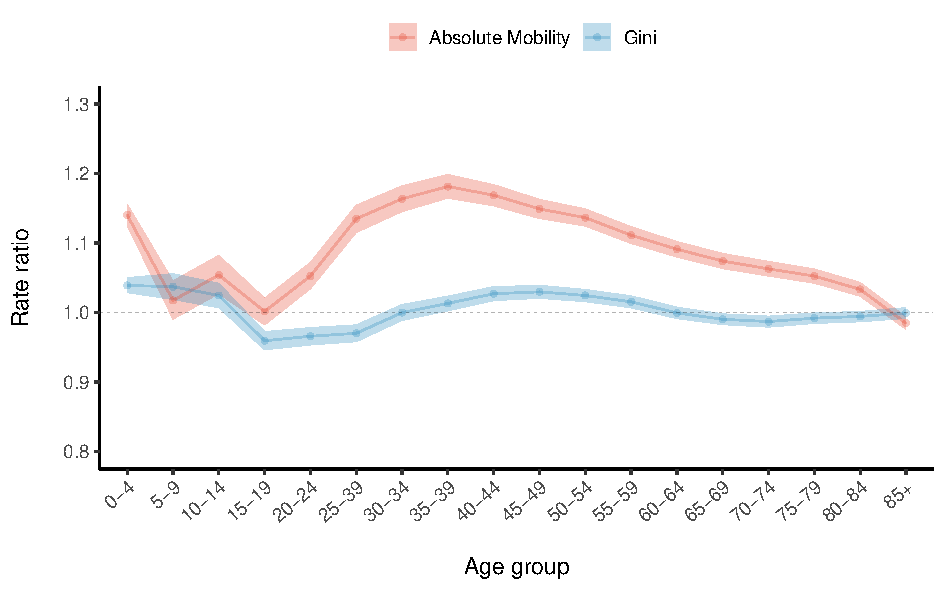
\includegraphics[width=1\textwidth]{figures/files/w4_effects_age_pcprior_1_10_abs.pdf}
  \end{subfigure}%

 \begin{subfigure}[b]{.60\linewidth}
   \caption{Men}
    \centering
    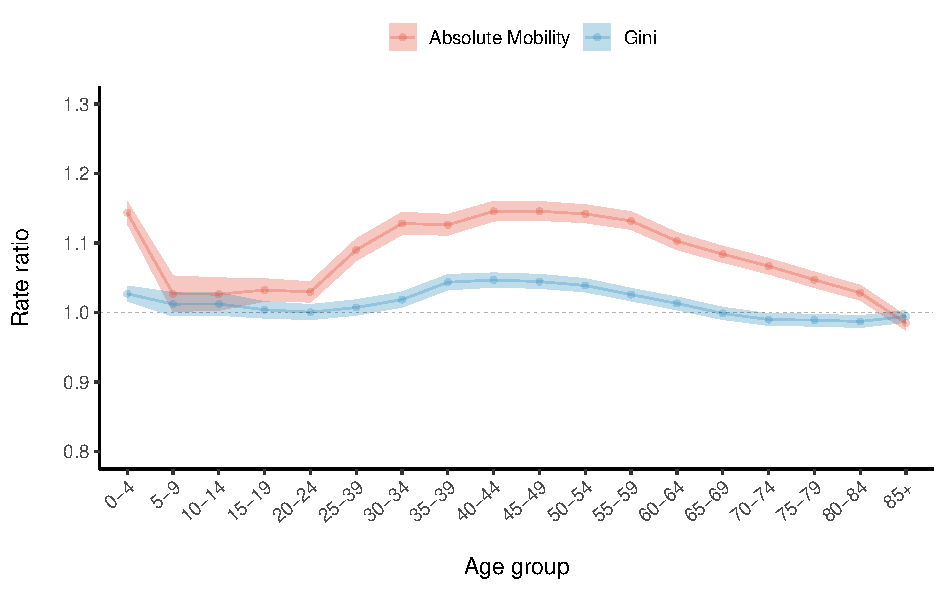
\includegraphics[width=1\textwidth]{figures/files/m4_effects_age_pcprior_1_10_abs.pdf}
  \end{subfigure}%
  \label{fig:effects_age_abs}
\end{figure}


\newpage
\begin{figure}[htp]
\caption{95\% Credibility Interval of Predicted LE Differences 
\newline by Age Group, Increase in One Standard Deviation
\newline Model \textit{Covariates} in Tables \ref{tbl:w_age_pcprior_1_10_abs} and \ref{tbl:m_age_pcprior_1_10_abs}}
\centering

  \begin{subfigure}[b]{.60\linewidth}
    \centering
       \caption{Women}
    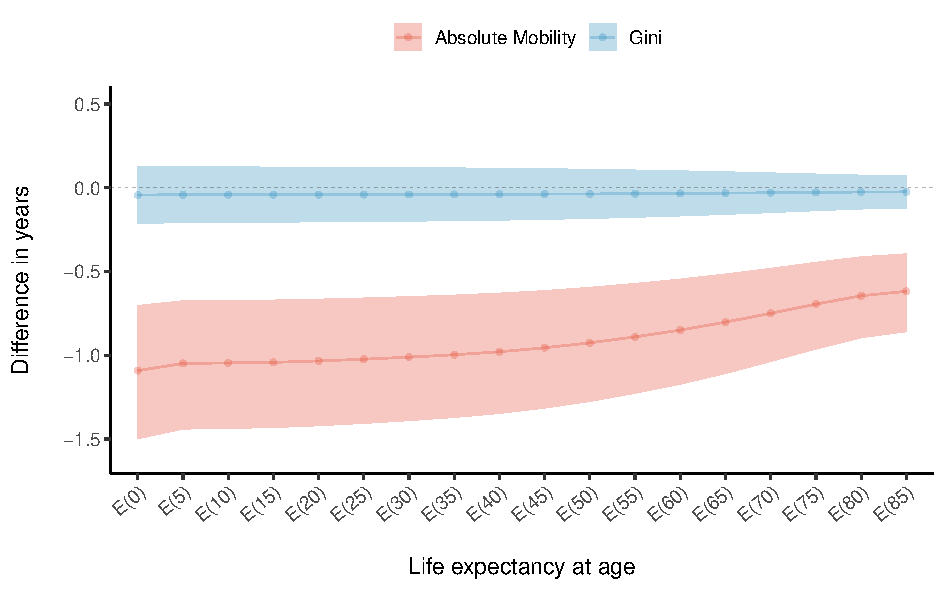
\includegraphics[width=1\textwidth]{figures/files/w4_le_differences_pcprior_1_10_abs.pdf}
  \end{subfigure}%

 \begin{subfigure}[b]{.60\linewidth}
   \caption{Men}
    \centering
    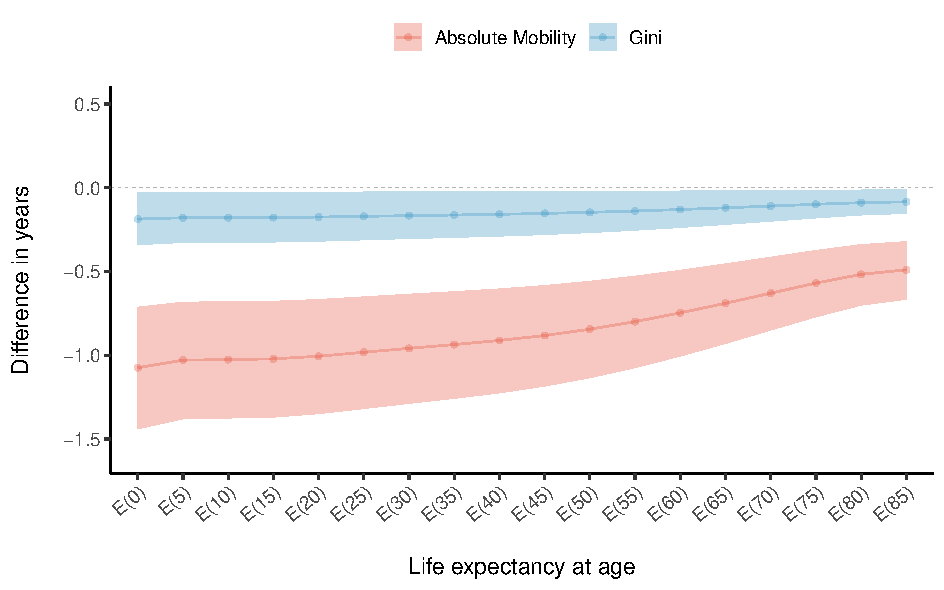
\includegraphics[width=1\textwidth]{figures/files/m4_le_differences_pcprior_1_10_abs.pdf}
  \end{subfigure}%
  \label{fig:le_differences_abs}
\end{figure}


\newpage
\begin{figure}[htp]
\caption{95\% Credibility Interval of Predicted Relative LE Differences 
\newline by Age Group, Increase in One Standard Deviation
\newline Model \textit{Covariates}  in Tables \ref{tbl:w_age_pcprior_1_10_abs} and \ref{tbl:m_age_pcprior_1_10}}
\centering

  \begin{subfigure}[b]{.60\linewidth}
    \centering
       \caption{Women}
    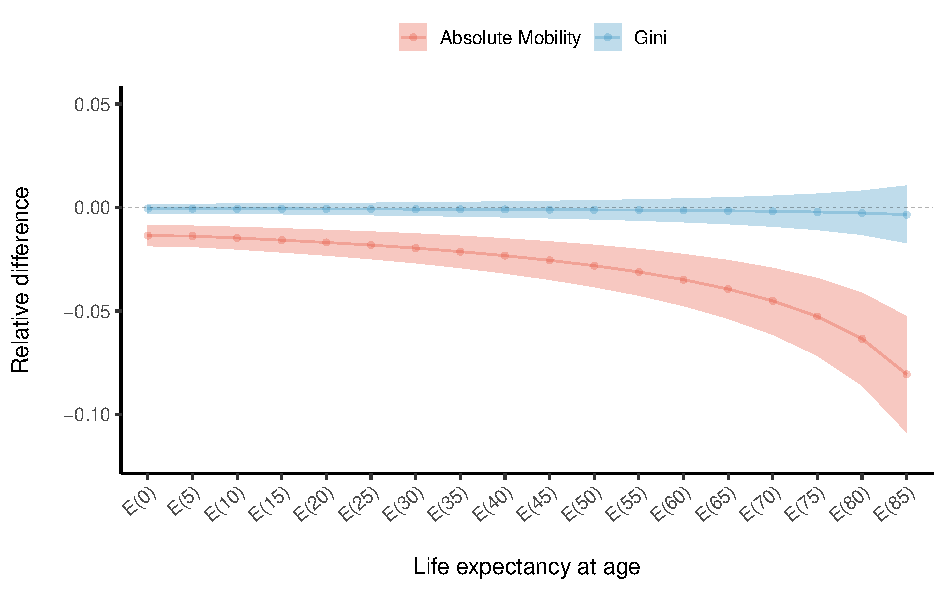
\includegraphics[width=1\textwidth]{figures/files/w4_le_re_differences_pcprior_1_10_abs.pdf}
  \end{subfigure}%

 \begin{subfigure}[b]{.60\linewidth}
   \caption{Men}
    \centering
    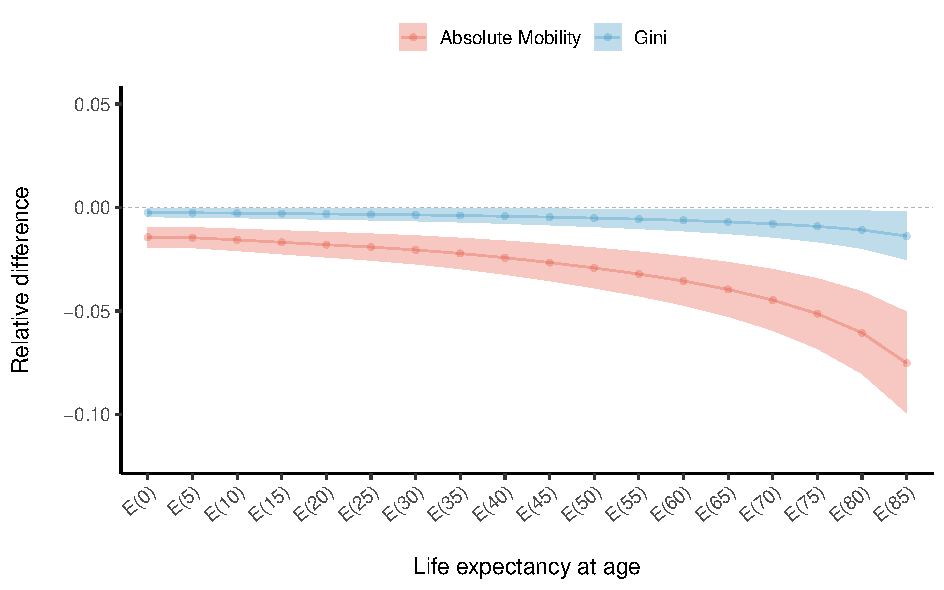
\includegraphics[width=1\textwidth]{figures/files/m4_le_re_differences_pcprior_1_10_abs.pdf}
  \end{subfigure}%
  \label{fig:le_re_differences_abs}
\end{figure}

\newpage
\begin{figure}[htp]
\caption{Posterior Distribution $exp(\beta_m)$ and $exp(\beta_g)$
\newline Model \textit{Covariates}}
\centering

  \begin{subfigure}[b]{.80\linewidth}
    \centering
       \caption{Women}
    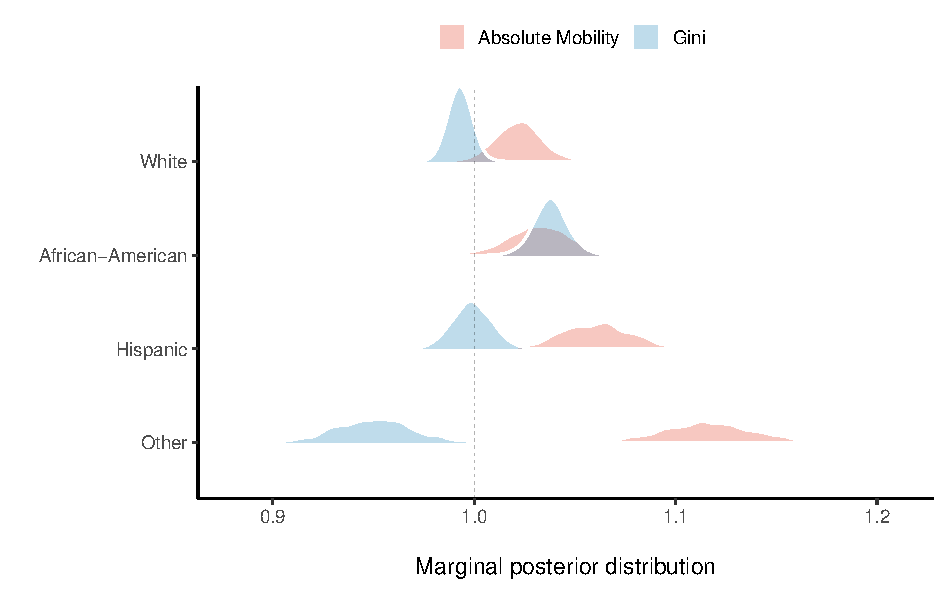
\includegraphics[width=1\textwidth]{figures/files/w_race_dist_pcprior_1_10_abs.pdf}
  \end{subfigure}%

 \begin{subfigure}[b]{.80\linewidth}
   \caption{Men}
    \centering
    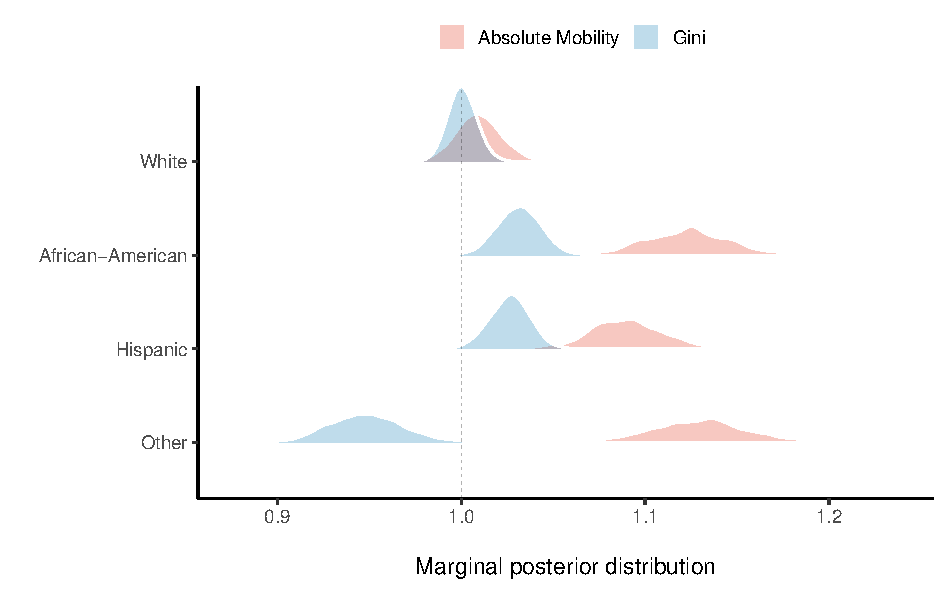
\includegraphics[width=1\textwidth]{figures/files/m_race_dist_pcprior_1_10_abs.pdf}
  \end{subfigure}%
  \label{fig:race_abs}
\end{figure}

\newpage
\begin{figure}[htp]
\caption{95\% Credibility Interval of Predicted LE Differences  \newline 
 by Age Group and Race/Ethnicity, Increase in One Standard Deviation}
\centering

  \begin{subfigure}[b]{.45\linewidth}
    \centering
       \caption{Women - Absolute Mobility}
    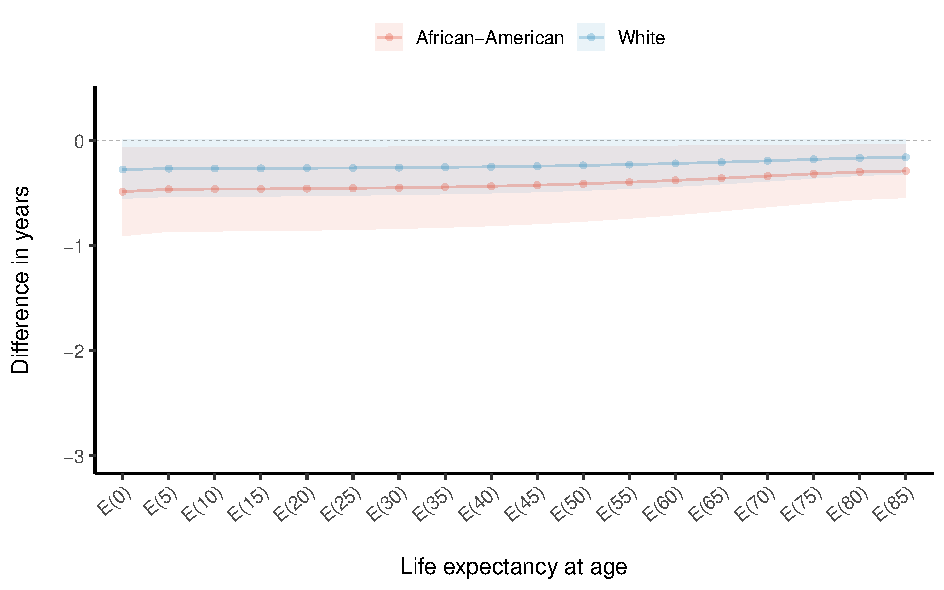
\includegraphics[width=1\textwidth]{figures/files/w_le_differences_race_mob_pcprior_1_10_abs.pdf}%
    ~
  \end{subfigure}
  \begin{subfigure}[b]{.45\linewidth}
    \centering
       \caption{Men - Absolute Mobility}
    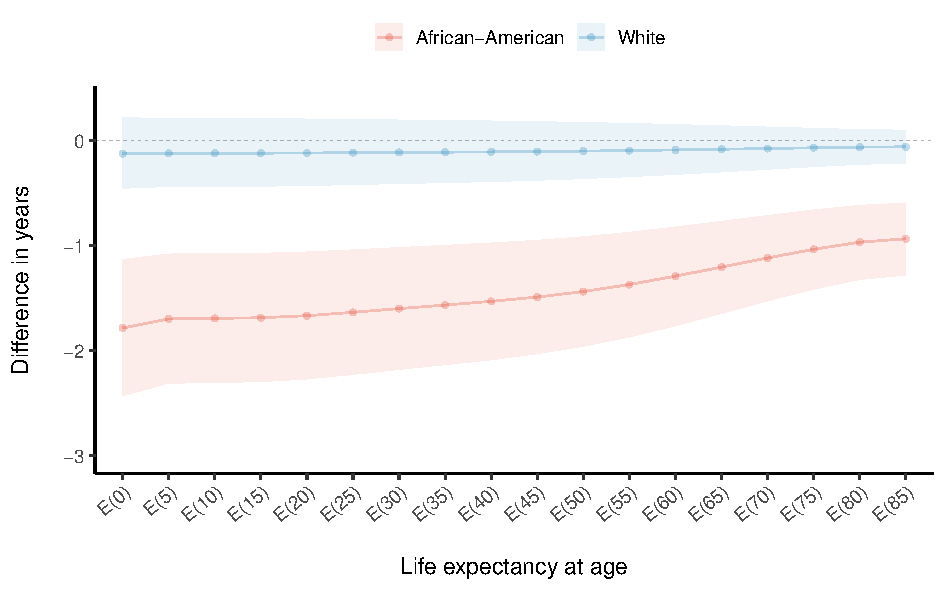
\includegraphics[width=1\textwidth]{figures/files/m_le_differences_race_mob_pcprior_1_10_abs.pdf}
  \end{subfigure}%
  
  \begin{subfigure}[b]{.45\linewidth}
    \centering
       \caption{Women - Gini}
    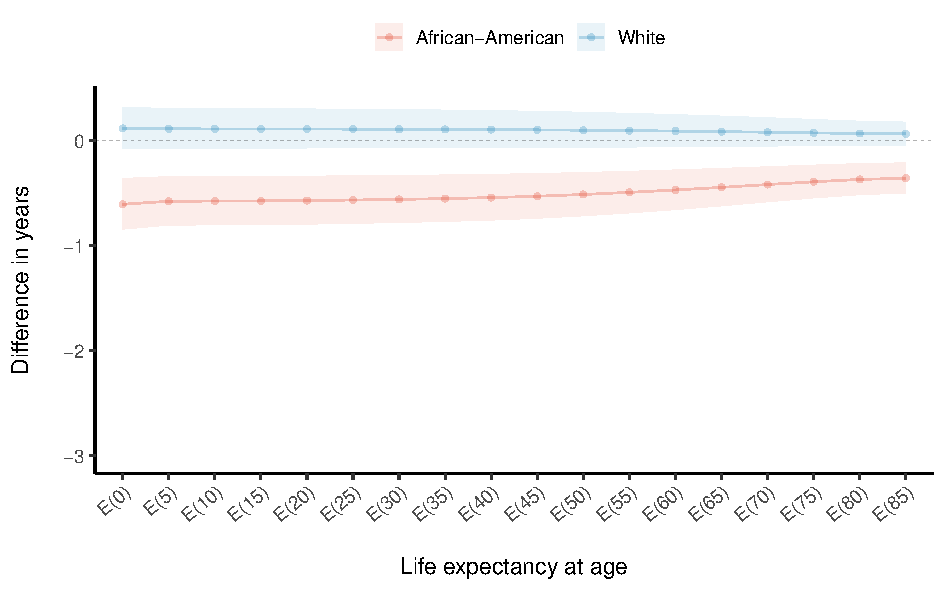
\includegraphics[width=1\textwidth]{figures/files/w_le_differences_race_gini_pcprior_1_10.pdf}
  \end{subfigure}
  \begin{subfigure}[b]{.45\linewidth}
    \centering
       \caption{Men - Gini}
    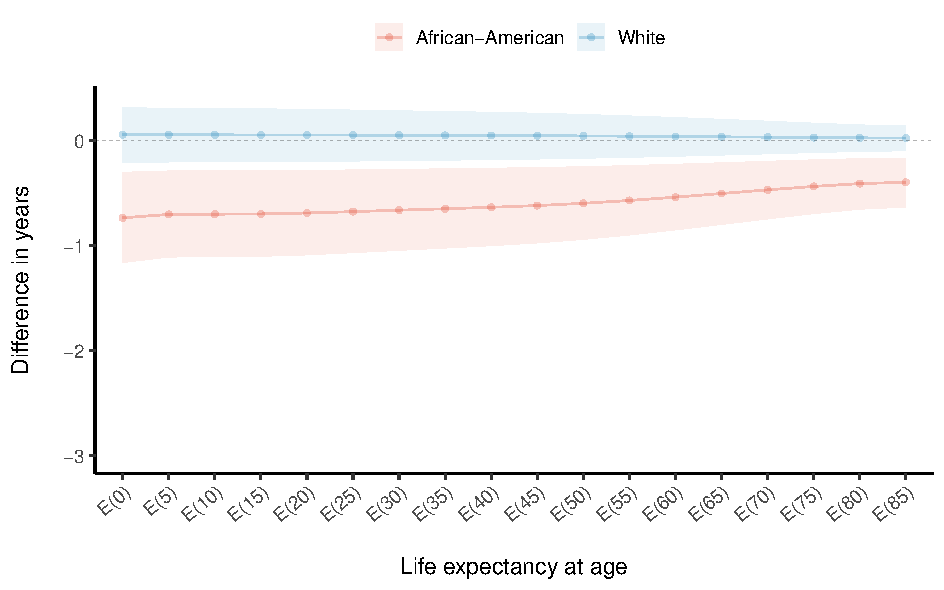
\includegraphics[width=1\textwidth]{figures/files/m_le_differences_race_gini_pcprior_1_10.pdf}
  \end{subfigure}%
  \label{fig:le_differences_age_race_abs}
\end{figure}

\newpage
\begin{figure}[htp]
\caption{95\% Credibility Interval of Predicted LE Relative Differences  \newline 
 by Age Group and Race/Ethnicity, Increase in One Standard Deviation}
\centering

  \begin{subfigure}[b]{.45\linewidth}
    \centering
       \caption{Women - Absolute Mobility}
    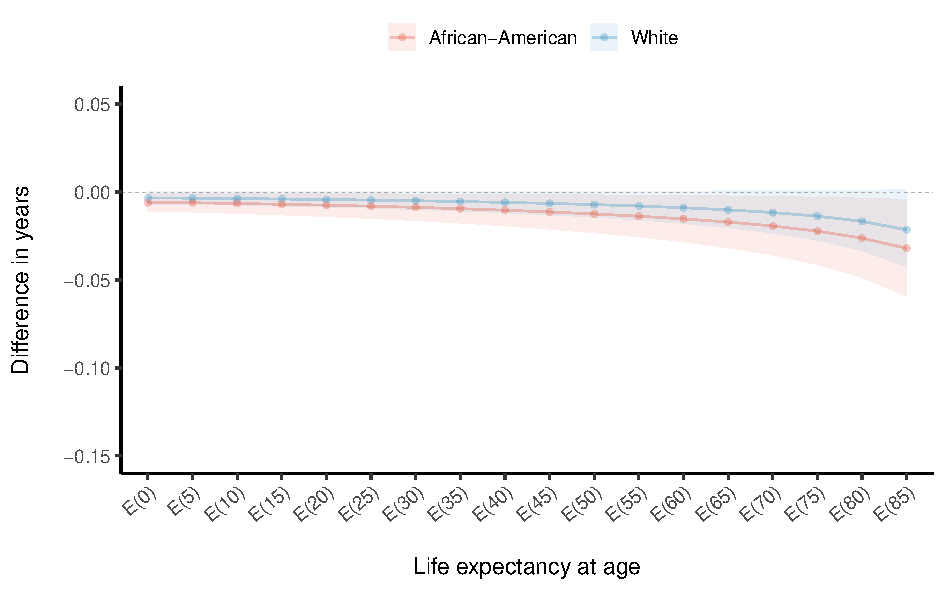
\includegraphics[width=1\textwidth]{figures/files/w_le_re_differences_race_mob_pcprior_1_10_abs.pdf}%
    ~
  \end{subfigure}
  \begin{subfigure}[b]{.45\linewidth}
    \centering
       \caption{Men - Absolute Mobility}
    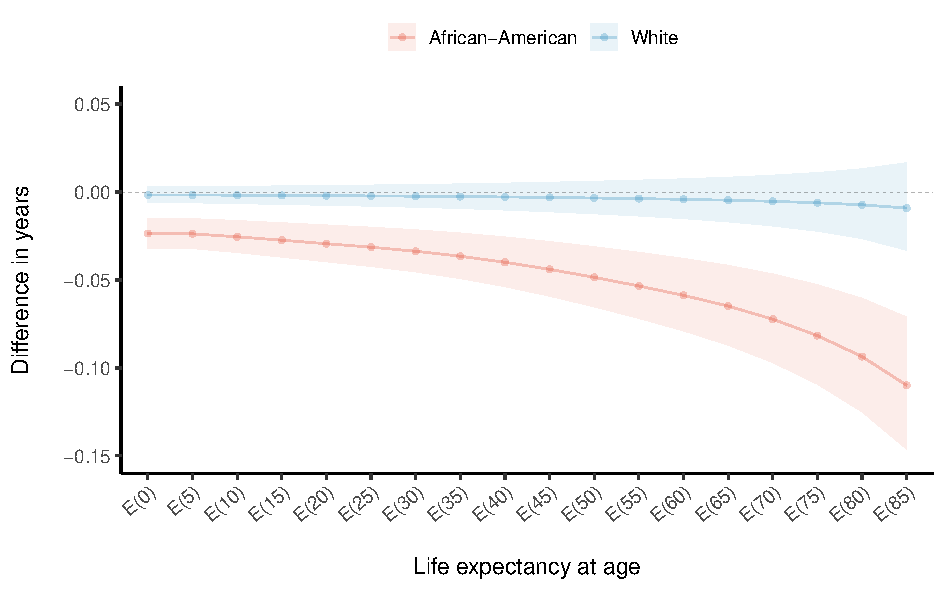
\includegraphics[width=1\textwidth]{figures/files/m_le_re_differences_race_mob_pcprior_1_10_abs.pdf}
  \end{subfigure}%
  
  \begin{subfigure}[b]{.45\linewidth}
    \centering
       \caption{Women - Gini}
    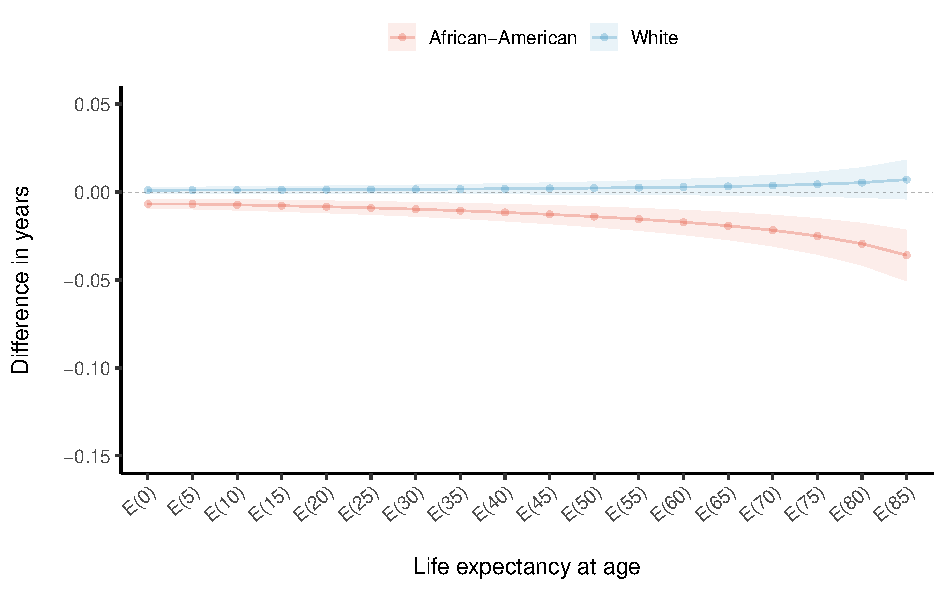
\includegraphics[width=1\textwidth]{figures/files/w_le_re_differences_race_gini_pcprior_1_10_abs.pdf}
  \end{subfigure}
  \begin{subfigure}[b]{.45\linewidth}
    \centering
       \caption{Men - Gini}
    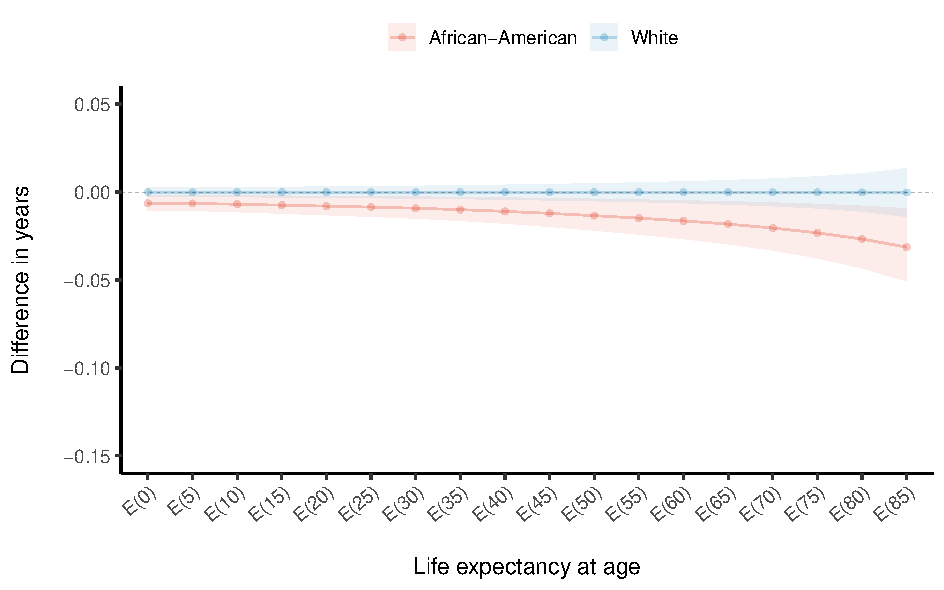
\includegraphics[width=1\textwidth]{figures/files/m_le_re_differences_race_gini_pcprior_1_10_abs.pdf}
  \end{subfigure}%
  \label{fig:le_re_differences_age_race_abs}
\end{figure}

\newpage
\begin{figure}[htp]
\caption{Posterior Distribution $exp(\beta_{\text{Mob}})$ and $exp(\beta{\text{Gini}})$ \newline by Cause of Death and Gender}
\centering

  \begin{subfigure}[b]{.80\linewidth}
    \centering
       \caption{Women}
    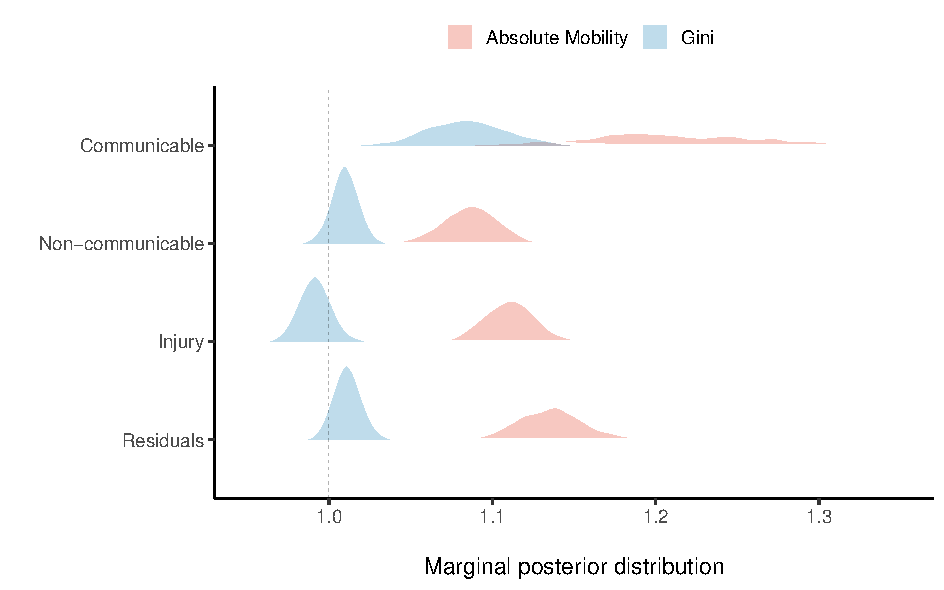
\includegraphics[width=1\textwidth]{figures/files/w_cause_dist_pcprior_1_10_abs.pdf}
  \end{subfigure}%

 \begin{subfigure}[b]{.80\linewidth}
   \caption{Men}
    \centering
    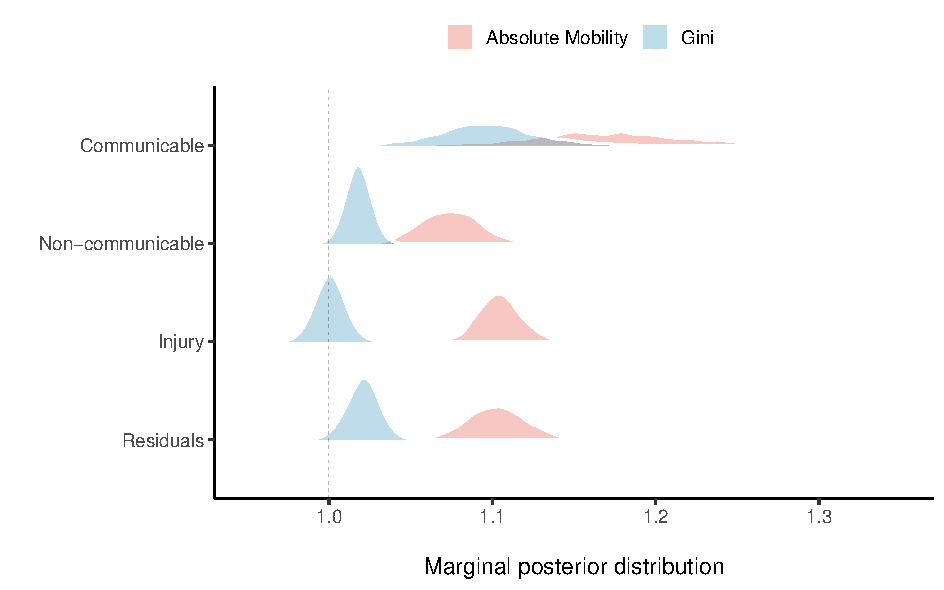
\includegraphics[width=1\textwidth]{figures/files/m_cause_dist_pcprior_1_10_abs.pdf}
  \end{subfigure}%
  \label{fig:cause_of_death_abs}
\end{figure}


\clearpage
\subsection{Cause of Death Coding}
\renewcommand{\arraystretch}{1.0}
\scriptsize

\begin{longtable}{lp{11cm}}

\caption{Code for Causes of Death, CDC} \label{tbl:cause_codes} \\
\hline
\addlinespace
\addlinespace
\textbf{Code CDC Database} & \textbf{Cause Title and ICD-10 Codes} \\
\addlinespace
\addlinespace
\hline
\addlinespace
\addlinespace
\multicolumn{2}{l}{\textbf{Group 1}} \\
\addlinespace
001 & Tuberculosis (A16A19) \\
002 & Syphilis (A50A53) \\
003 & Human immunodeficiency virus (HIV) disease (B20B24) \\
027 & Influenza and pneumonia (J10J18) \\
\addlinespace
\addlinespace

\multicolumn{2}{l}{\textbf{Group 2}} \\
\addlinespace
004 & Malignant neoplasms (C00C97) \\
005 & Malignant neoplasm of stomach (C16) \\
006 & Malignant neoplasms of colon, rectum and anus (C18C21) \\
007 & Malignant neoplasm of pancreas (C25) \\
008 & Malignant neoplasms of trachea, bronchus and lung (C33C34) \\
009 & Malignant neoplasm of breast (C50) \\
010 & Malignant neoplasms of cervix uteri, corpus uteri and ovary (C53C56) \\
011 & Malignant neoplasm of prostate (C61) \\
012 & Malignant neoplasms of urinary tract (C64C68) \\
013 & NonHodgkin's lymphoma (C82C85) \\
014 & Leukemia (C91C95) \\
015 & Other malignant neoplasms (C00C15, C17, C22C24,  C26C32, C37C49, C51C52, C57C60, C62C63, C69C81, C88, C90, C96C97) \\
\addlinespace
016 & Diabetes mellitus (E10E14) \\
017 & Alzheimer's disease (G30) \\
028 & Chronic lower respiratory diseases (J40J47) \\
035 & Sudden infant death syndrome (R95) \\
029 & Peptic ulcer (K25K28) \\
030 & Chronic liver disease and cirrhosis (K70,K73K74) \\
031 & Nephritis, nephrotic syndrome, and nephrosis (N00N07,N17N19,N25N27) \\
032 & Pregnancy, childbirth and the puerperium (O00O99) \\
033 & Certain conditions originating in the perinatal period (P00P96) \\
034 & Congenital malformations, deformations and chromosomal abnormalities (Q00Q99) \\
036 & Symptoms, signs and abnormal clinical and laboratory findings, not elsewhere classified (excluding sudden infant death syndrome) (R00R94,R96R99) \\
018 & Major cardiovascular diseases (I00I78) \\
019 & Diseases of heart (I00I09,I11,I13,I20I51) \\
020 & Hypertensive heart disease with or without renal disease (I11,I13) \\
021 & Ischemic heart diseases (I20I25) \\
022 & Other diseases of heart (I00I09,I26I51) \\
023 & Essential (primary) hypertension and hypertensive renal disease (I10,I12) \\
024 & Cerebrovascular diseases (I60I69) \\
025 & Atherosclerosis (I70) \\
026 & Other diseases of circulatory system (I71I78) \\
\addlinespace
\addlinespace
\multicolumn{2}{l}{\textbf{Group 3}} \\
\addlinespace
038 & Motor vehicle accidents (V02V04, V09.0, V12V14, V19.0V19.2, V19.4V19.6, V20V79, V80.3V80.5, V81.0V81.1, V82.0V82.1, V83V86,V87.0V87.8, V88.0V88.8, V89.0,V89.2) \\
039 & All other and unspecified accidents and adverse effects (V01, V05V06, V09.1, V09.3V09.9, V10V11,V15V18, V19.3,V19.8V19.9, V80.0V80.2, V80.6V80.9, V81.2V81.9, V82.2V82.9, V87.9, V88.9,V89.1, V89.3,V89.9, V90X59, Y40Y86, Y88) \\
042 & All other external causes (Y10Y36, Y87.2, Y89) \\
040 & Intentional self-harm (suicide) (*U03, X60X84, Y87.0) \\
041 & Assault (homicide) (*U01-*U02, X85Y09, Y87.1) \\
\addlinespace
\addlinespace
\multicolumn{2}{l}{\textbf{Group 4}} \\
\addlinespace
037 & All other diseases (Residual) (A00A09, A20A49, A54B19, B25B99, D00E07, E15G25, G31H93, I80J06, J20J39, J60K22, K29K66, K71K72, K75M99, N10N15, N20N23, N28N98) \\
\addlinespace
\addlinespace
\hline
\end{longtable}

%TC:endignore

\end{document}


